\documentclass{beamer}
\usepackage{amsmath}
\usepackage{graphicx}
\usepackage{url}
%\usepackage{fancyvrb}
\usepackage{color}
\usepackage{tikz}
%\usepackage{movie15}
\usepackage{multimedia}
\usepackage{hyperref}
\usepackage{subfigure}

%\newcommand{\opal}{\textsc{OPAL}}
\newcommand{\opalt}{\textsc{OPAL-t }}
\newcommand{\opalcycl}{\textsc{OPAL-cycl}}
\newcommand{\opalmap}{\textsc{OPAL-map }}
\newcommand{\opalenv}{\textsc{OPAL-envelop}}

\newcommand{\mad}{\textsc{mad }}
\newcommand{\madnine}{\textsc{mad9 }}
\newcommand{\madninep}{\textsc{mad9p }}
\newcommand{\madeight}{\textsc{mad8 }}

\newcommand{\classic}{\textsc{classic }}
\newcommand{\hfifepart}{\textsc{H5Part }}
\newcommand{\hfifefe}{\textsc{H5FED }}

\renewcommand{\epsilon}{\varepsilon} 
\renewcommand{\vec}[1]{{\bf #1}} 
\newcommand{\dt}[1]{\frac{\partial #1}{\partial t}}
\newcommand{\dtt}[1]{\frac{\partial^2 #1}{\partial t^2}}
\newcommand{\dtvec}[1]{\frac{\partial {\mathbf #1}}{\partial t}}
\newcommand{\dttvec}[1]{\frac{\partial^2 {\mathbf #1}}{\partial t^2}}
\newcommand{\rot}{\vec{\nabla} \wedge }
\renewcommand{\div}{\vec{\nabla} \cdot }

\def\vec#1{\mathbf{#1}}
\def\vecg#1{\boldsymbol{#1}}
\def\norm#1{\| #1 \|} 
\def\tr{^{\!\top}}

\def\curl{{\bf curl}\,}
\def\curlp{{\rm curl}_p\,}
\def\div{{\rm div}\,}
\def\grad{\nabla}
\def\gradp{\nabla_p}
\def\dotp#1#2{\langle#1,#2\rangle}
\def\eps{\varepsilon}

\newcommand{\mat}[1]{\ensuremath{\boldsymbol{#1}}}
\newcommand{\vect}[1]{\ensuremath{\mathbf{#1}}}
\newcommand{\iprod}[2]{\ensuremath{\langle#1,#2\rangle}}
\newcommand{\abs}[1]{\ensuremath{|#1|}}

\newcommand{\Nedelec}{N\'{e}d\'{e}lec}

\newcommand{\id}[1]{\structure{#1}}

\newcommand {\Co}{{\mathbb{C}}}
\newcommand {\Int}{{\mathbb{Z}}}
\newcommand {\Nat}{{\mathbb{N}}}
%
%
\newcommand {\Hcurl}{{H(\mathbf{curl};\Omega)}}
\newcommand {\Hocurl}{{H_0(\mathbf{curl};\Omega)}}
\newcommand {\Hdiv}{{H(\mathrm{div};\Omega)}}
\newcommand {\Hodiv}{{H_0(\mathbf{div};\Omega)}}
%
\renewcommand {\Re}{{\rm I \kern-2pt R}}
\newcommand{\vc}[1]{\mbox{\boldmath $#1$}}
\newcommand {\RM}[1]{\mathrm{#1}}


\usetikzlibrary{shapes,arrows}

% This is the file main.tex
\mode<presentation>
{
  \usetheme{Warsaw}
  % or ...

  \setbeamercovered{transparent}
  % or whatever (possibly just delete it)
}
\usepackage[english]{babel}
% or whatever

\usepackage[latin1]{inputenc}
% or whatever

\usepackage{times}
\usepackage[T1]{fontenc}
\title[The Dark-current and Multipacting Simulation Capability of OPAL]{The Dark-current and Multipacting Simulation Capability of OPAL\\ - Modeling, Benchmarking and Application
 }
\author[Chuan et.al]{Ch. Wang, A. Adelmann, Y. Ineichen}
\date{\today}
\AtBeginSubsection[]
{
  \begin{frame}<beamer>{Outline}
    \tableofcontents[currentsection,currentsubsection]
  \end{frame}
}

\begin{document}
\begin{frame}
\titlepage
\end{frame}
%\begin{frame}{Outline}
%  \tableofcontents
  % You might wish to add the option [pausesections]
%\end{frame}
%\section*{Outlines}
\begin{frame}
\tableofcontents
\end{frame}
\section{Background and Goal}
\subsection{Dark current and Multipacting Phenomenas}
\begin{frame}
\frametitle{Experimental Observations}
\begin{columns}
\begin{column}[t]{7cm}
\begin{figure}[H]
\begin{center}
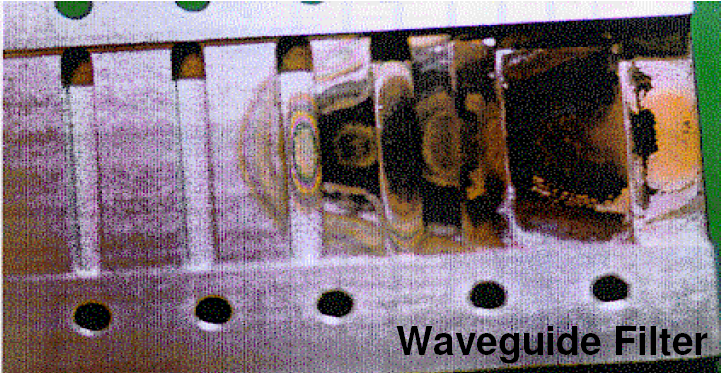
\includegraphics[width=1\textwidth]{Screenshot.png}
%\scalebox{0.7}{
\begin{tikzpicture}
\usetikzlibrary{arrows}
\draw [->,black,-latex] (-1.5,0) -- (1.5,0);
\draw [->,black,-latex] (-1.5,0) -- (-1.5,2);
\draw (1.5,0) -- (0.0,2);
\draw  [<-,black,latex-](0.0,2) -- (-1.5,0.0);
\draw [->,black,-latex,dashed] (-1.5,0) -- (0.5,0.5);
\node[below] (w) at (-0.15,0.5) {$\vec{w}$};
\draw[dashed] (0.5,0.5) -- (-1.18,0.5);
\draw[dashed] (0.5,0.5) -- (0.01,0.0);
\node[above] (ti) at (-1.18,0.5) {$t_i$};
\node[below] (si) at (0.01,0.0) {$s_i$};
\node[above] (t0) at (-1.7,0.) {$\mathbf{t_0}$};
\node[right] (t1) at (1.5,0) {$\mathbf{t_1}$};
\node[above] (t2) at (0.0,2.0) {$\mathbf{t_2}$};
\node[above] (n) at (-1.5,2) {$\vec{n}$};
\node[above] (v) at (-0.5,1.5) {$\vec{v}$};
\node[below] (u) at (1.2,0.0) {$\vec{u}$};
\path[draw=black,fill=black] (0.0,2.0) circle (2pt);
\path[draw=black,fill=black] (1.5,0.0) circle (2pt);
\path[draw=black,fill=black] (-1.5,0.0) circle (2pt);
\draw (-3.5,-1) -- (2.5,-1);
\draw (2.5,-1) -- (5,3);
\draw (0,3) -- (5,3);
\draw (-3.5,-1) -- (0,3);
\draw (0.5,0.5) -- (1.6,5);
\path[draw=black] (0.5,0.5) circle (2pt);
\node[above] (I) at (0.5,0.5) {$\mathbf{I}$};
\node[right] (x0) at (1.6,5) {$\mathbf{x_0}$};
\draw[dashed] (0.5,0.5) -- (-0.1,-1.9);
\node[right] (x1) at (0.0,-1.9) {$\mathbf{x_1}$};
\node[right] (ri) at (1,2.5) {$r_i$};
\path[draw=black,fill=black] (-0.1,-1.9) circle (2pt);
\path[draw=black,fill=black] (1.6,5) circle (2pt);
\end{tikzpicture}
}
\end{center}
\end{figure}
\end{column}
\begin{column}[t]{5.7cm}
\begin{figure}[H]
\begin{center}
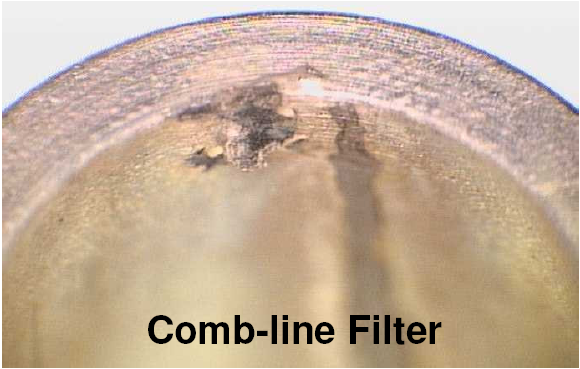
\includegraphics[width=1\textwidth]{Screenshot_0.png}
%\scalebox{0.7}{
\begin{tikzpicture}
\usetikzlibrary{arrows}
\draw [->,black,-latex] (-1.5,0) -- (1.5,0);
\draw [->,black,-latex] (-1.5,0) -- (-1.5,2);
\draw (1.5,0) -- (0.0,2);
\draw  [<-,black,latex-](0.0,2) -- (-1.5,0.0);
\draw [->,black,-latex,dashed] (-1.5,0) -- (0.5,0.5);
\node[below] (w) at (-0.15,0.5) {$\vec{w}$};
\draw[dashed] (0.5,0.5) -- (-1.18,0.5);
\draw[dashed] (0.5,0.5) -- (0.01,0.0);
\node[above] (ti) at (-1.18,0.5) {$t_i$};
\node[below] (si) at (0.01,0.0) {$s_i$};
\node[above] (t0) at (-1.7,0.) {$\mathbf{t_0}$};
\node[right] (t1) at (1.5,0) {$\mathbf{t_1}$};
\node[above] (t2) at (0.0,2.0) {$\mathbf{t_2}$};
\node[above] (n) at (-1.5,2) {$\vec{n}$};
\node[above] (v) at (-0.5,1.5) {$\vec{v}$};
\node[below] (u) at (1.2,0.0) {$\vec{u}$};
\path[draw=black,fill=black] (0.0,2.0) circle (2pt);
\path[draw=black,fill=black] (1.5,0.0) circle (2pt);
\path[draw=black,fill=black] (-1.5,0.0) circle (2pt);
\draw (-3.5,-1) -- (2.5,-1);
\draw (2.5,-1) -- (5,3);
\draw (0,3) -- (5,3);
\draw (-3.5,-1) -- (0,3);
\draw (0.5,0.5) -- (1.6,5);
\path[draw=black] (0.5,0.5) circle (2pt);
\node[above] (I) at (0.5,0.5) {$\mathbf{I}$};
\node[right] (x0) at (1.6,5) {$\mathbf{x_0}$};
\draw[dashed] (0.5,0.5) -- (-0.1,-1.9);
\node[right] (x1) at (0.0,-1.9) {$\mathbf{x_1}$};
\node[right] (ri) at (1,2.5) {$r_i$};
\path[draw=black,fill=black] (-0.1,-1.9) circle (2pt);
\path[draw=black,fill=black] (1.6,5) circle (2pt);
\end{tikzpicture}
}
\end{center}
\end{figure}
\end{column}
\end{columns}
\begin{itemize}
\item see Ref ~\cite{SPACE};
\end{itemize}
\end{frame}
\begin{frame}
\frametitle{Experimental Observations}
\begin{columns}
\begin{column}[t]{7cm}
\begin{figure}[H]
\begin{center}
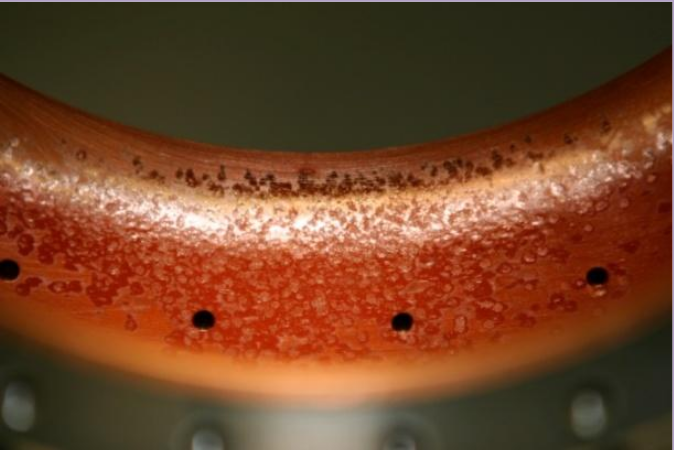
\includegraphics[width=1.\textwidth]{Screenshot-1.png}
%\scalebox{0.7}{
\begin{tikzpicture}
\usetikzlibrary{arrows}
\draw [->,black,-latex] (-1.5,0) -- (1.5,0);
\draw [->,black,-latex] (-1.5,0) -- (-1.5,2);
\draw (1.5,0) -- (0.0,2);
\draw  [<-,black,latex-](0.0,2) -- (-1.5,0.0);
\draw [->,black,-latex,dashed] (-1.5,0) -- (0.5,0.5);
\node[below] (w) at (-0.15,0.5) {$\vec{w}$};
\draw[dashed] (0.5,0.5) -- (-1.18,0.5);
\draw[dashed] (0.5,0.5) -- (0.01,0.0);
\node[above] (ti) at (-1.18,0.5) {$t_i$};
\node[below] (si) at (0.01,0.0) {$s_i$};
\node[above] (t0) at (-1.7,0.) {$\mathbf{t_0}$};
\node[right] (t1) at (1.5,0) {$\mathbf{t_1}$};
\node[above] (t2) at (0.0,2.0) {$\mathbf{t_2}$};
\node[above] (n) at (-1.5,2) {$\vec{n}$};
\node[above] (v) at (-0.5,1.5) {$\vec{v}$};
\node[below] (u) at (1.2,0.0) {$\vec{u}$};
\path[draw=black,fill=black] (0.0,2.0) circle (2pt);
\path[draw=black,fill=black] (1.5,0.0) circle (2pt);
\path[draw=black,fill=black] (-1.5,0.0) circle (2pt);
\draw (-3.5,-1) -- (2.5,-1);
\draw (2.5,-1) -- (5,3);
\draw (0,3) -- (5,3);
\draw (-3.5,-1) -- (0,3);
\draw (0.5,0.5) -- (1.6,5);
\path[draw=black] (0.5,0.5) circle (2pt);
\node[above] (I) at (0.5,0.5) {$\mathbf{I}$};
\node[right] (x0) at (1.6,5) {$\mathbf{x_0}$};
\draw[dashed] (0.5,0.5) -- (-0.1,-1.9);
\node[right] (x1) at (0.0,-1.9) {$\mathbf{x_1}$};
\node[right] (ri) at (1,2.5) {$r_i$};
\path[draw=black,fill=black] (-0.1,-1.9) circle (2pt);
\path[draw=black,fill=black] (1.6,5) circle (2pt);
\end{tikzpicture}
}
\end{center}
\end{figure}
\end{column}
\begin{column}[t]{5.1cm}
\begin{figure}[H]
\begin{center}
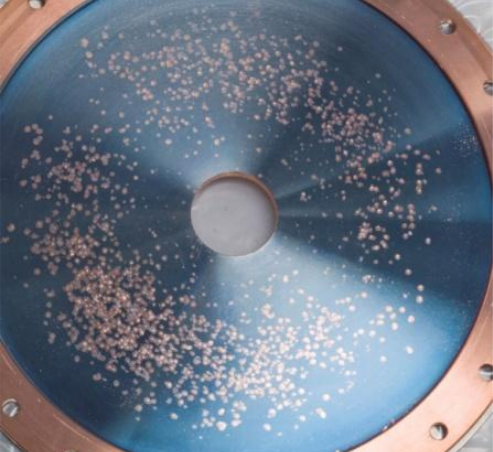
\includegraphics[width=1.\textwidth]{Screenshot-2.png}
%\scalebox{0.7}{
\begin{tikzpicture}
\usetikzlibrary{arrows}
\draw [->,black,-latex] (-1.5,0) -- (1.5,0);
\draw [->,black,-latex] (-1.5,0) -- (-1.5,2);
\draw (1.5,0) -- (0.0,2);
\draw  [<-,black,latex-](0.0,2) -- (-1.5,0.0);
\draw [->,black,-latex,dashed] (-1.5,0) -- (0.5,0.5);
\node[below] (w) at (-0.15,0.5) {$\vec{w}$};
\draw[dashed] (0.5,0.5) -- (-1.18,0.5);
\draw[dashed] (0.5,0.5) -- (0.01,0.0);
\node[above] (ti) at (-1.18,0.5) {$t_i$};
\node[below] (si) at (0.01,0.0) {$s_i$};
\node[above] (t0) at (-1.7,0.) {$\mathbf{t_0}$};
\node[right] (t1) at (1.5,0) {$\mathbf{t_1}$};
\node[above] (t2) at (0.0,2.0) {$\mathbf{t_2}$};
\node[above] (n) at (-1.5,2) {$\vec{n}$};
\node[above] (v) at (-0.5,1.5) {$\vec{v}$};
\node[below] (u) at (1.2,0.0) {$\vec{u}$};
\path[draw=black,fill=black] (0.0,2.0) circle (2pt);
\path[draw=black,fill=black] (1.5,0.0) circle (2pt);
\path[draw=black,fill=black] (-1.5,0.0) circle (2pt);
\draw (-3.5,-1) -- (2.5,-1);
\draw (2.5,-1) -- (5,3);
\draw (0,3) -- (5,3);
\draw (-3.5,-1) -- (0,3);
\draw (0.5,0.5) -- (1.6,5);
\path[draw=black] (0.5,0.5) circle (2pt);
\node[above] (I) at (0.5,0.5) {$\mathbf{I}$};
\node[right] (x0) at (1.6,5) {$\mathbf{x_0}$};
\draw[dashed] (0.5,0.5) -- (-0.1,-1.9);
\node[right] (x1) at (0.0,-1.9) {$\mathbf{x_1}$};
\node[right] (ri) at (1,2.5) {$r_i$};
\path[draw=black,fill=black] (-0.1,-1.9) circle (2pt);
\path[draw=black,fill=black] (1.6,5) circle (2pt);
\end{tikzpicture}
}
\end{center}
\end{figure}
\end{column}
\end{columns}
\begin{itemize}
\item see Ref ~\cite{Linac};
\end{itemize}
\end{frame}
\begin{frame}
\frametitle{Experimental Observations}
\begin{itemize}
\item Multipacting is a very disturbing phenomenon
appearing in high-Q RF cavities. Electrons are pulled
out from the walls of resonators by the RF voltage. By
hitting other metallic surfaces new electrons are
produced. This kind of discharge will limit the power
level until the surfaces will be cleaned through a
conditioning process. But this process is very time-consuming. \cite{cyclotron}
\end{itemize}
\end{frame}
\subsection{Existing Tools: Codes and Theory}
\begin{frame}
\frametitle{Codes Review}
\begin{figure}[H]
\begin{center}
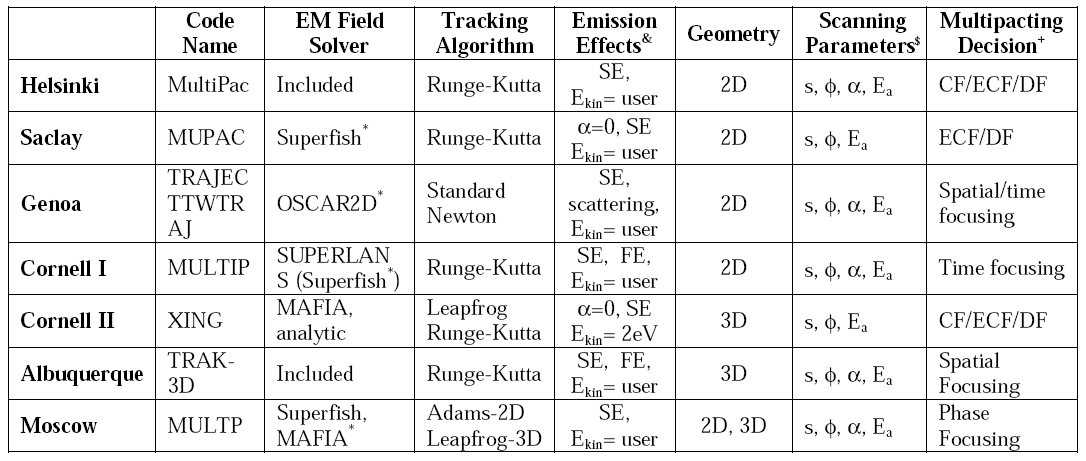
\includegraphics[width=1\textwidth]{Screenshot-4.png}
\end{center}
\end{figure}
\begin{itemize}
\item Most codes calculate electron trajectories and CF, ECF, DF.\ (severe multiplications) \cite{coderv}
\end{itemize}
\end{frame}
\begin{frame}[allowframebreaks]
\frametitle{Classic Multipacting Theory}
\begin{itemize}
\item Simple geometries (parallel plate, rectangular waveguide or coaxial line)
\item Deterministic: emission energy equals constant fraction of impact energy
\item Multipacting is contributed only by the electrons whose transit times through the gap are
equal to an odd number of half-periods of the high-frequency field
\end{itemize}
\begin{figure}[H]
\begin{center}
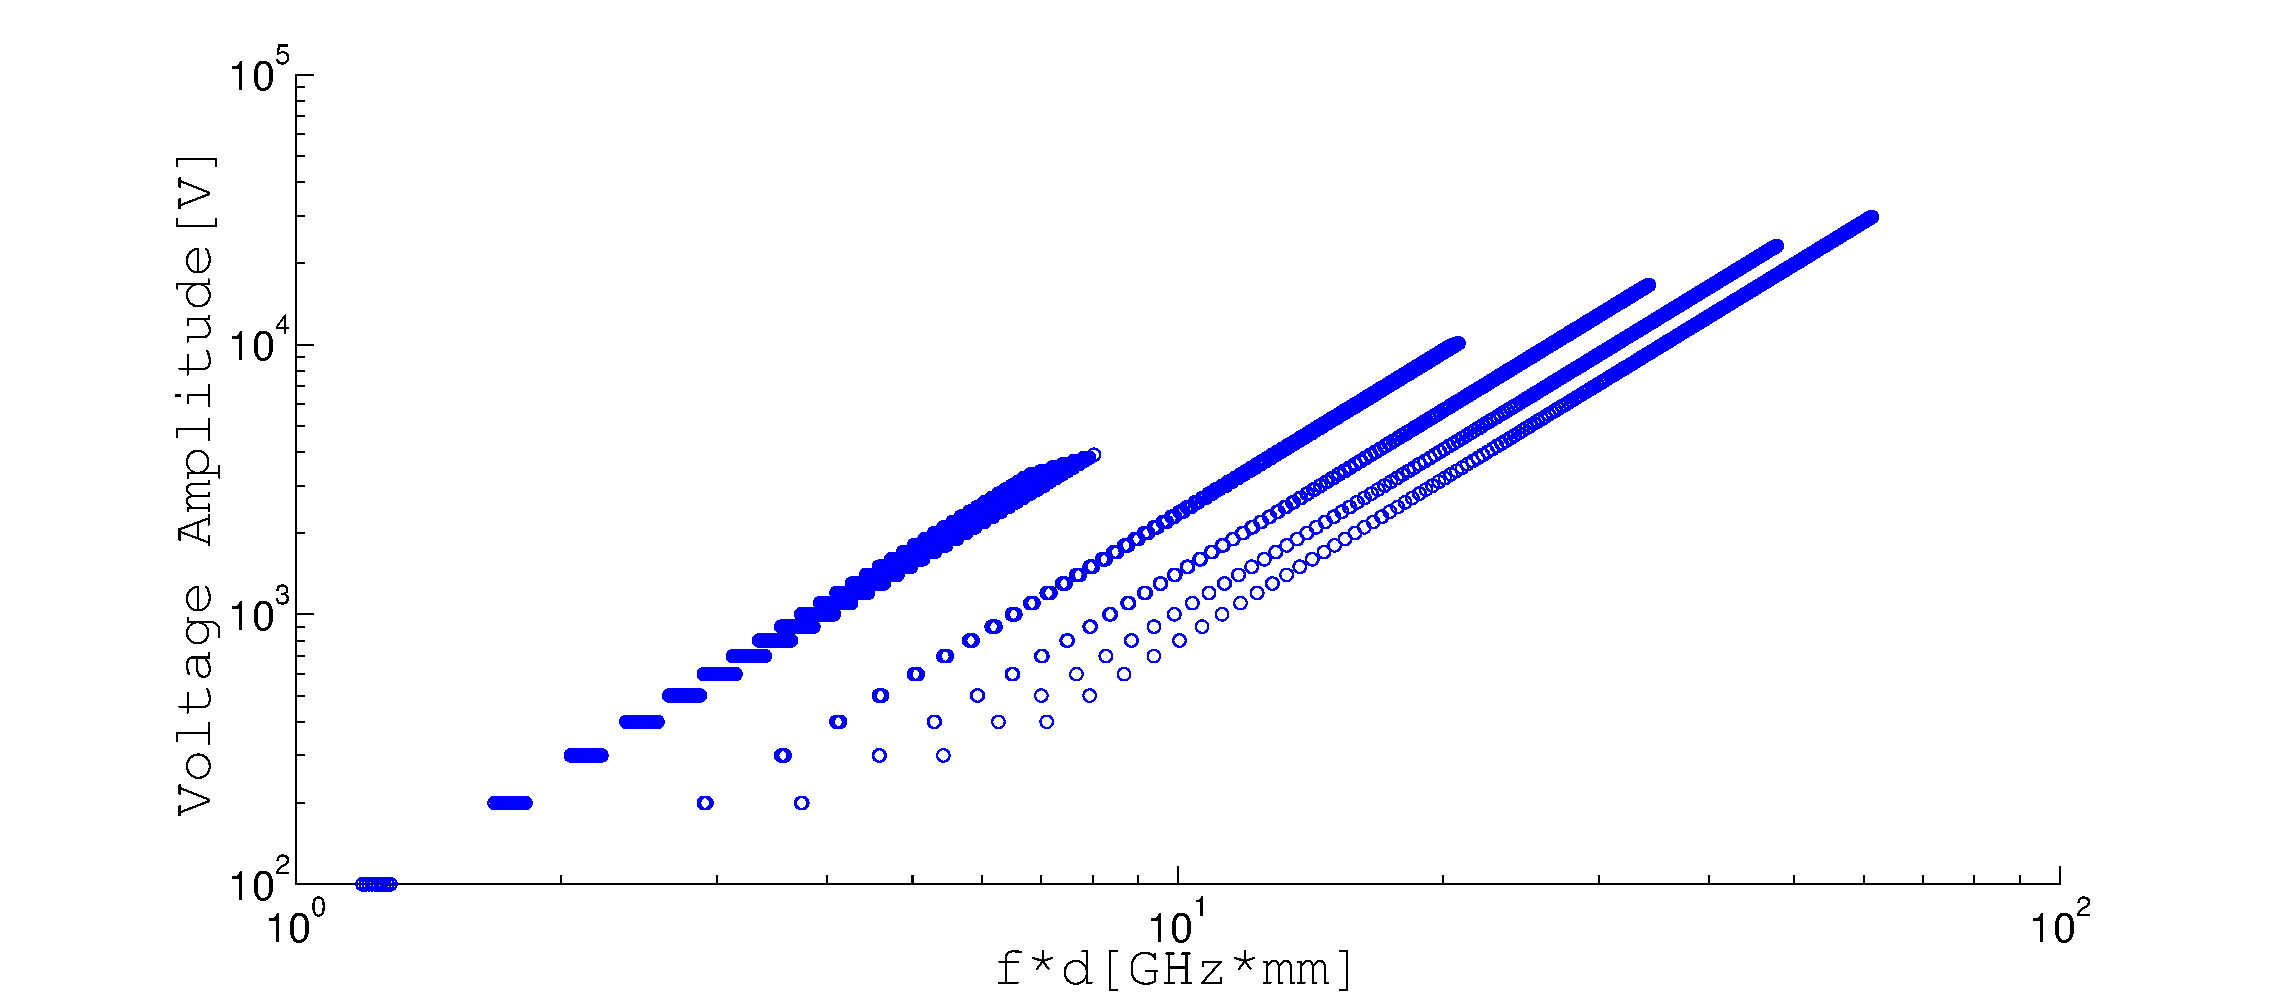
\includegraphics[width=1.0\textwidth]{right_unit.pdf}
%/Users/adelmann/svnwork/adelmann/papers/figures/Latex-Figures/Incident.tikz
\end{center}
%\caption{Line segment-triangle intersection()\label{fig:L-T}}
\end{figure}
\begin{itemize}
\item Example resonant zone in phase space
\end{itemize}
\begin{figure}[H]
\begin{center}
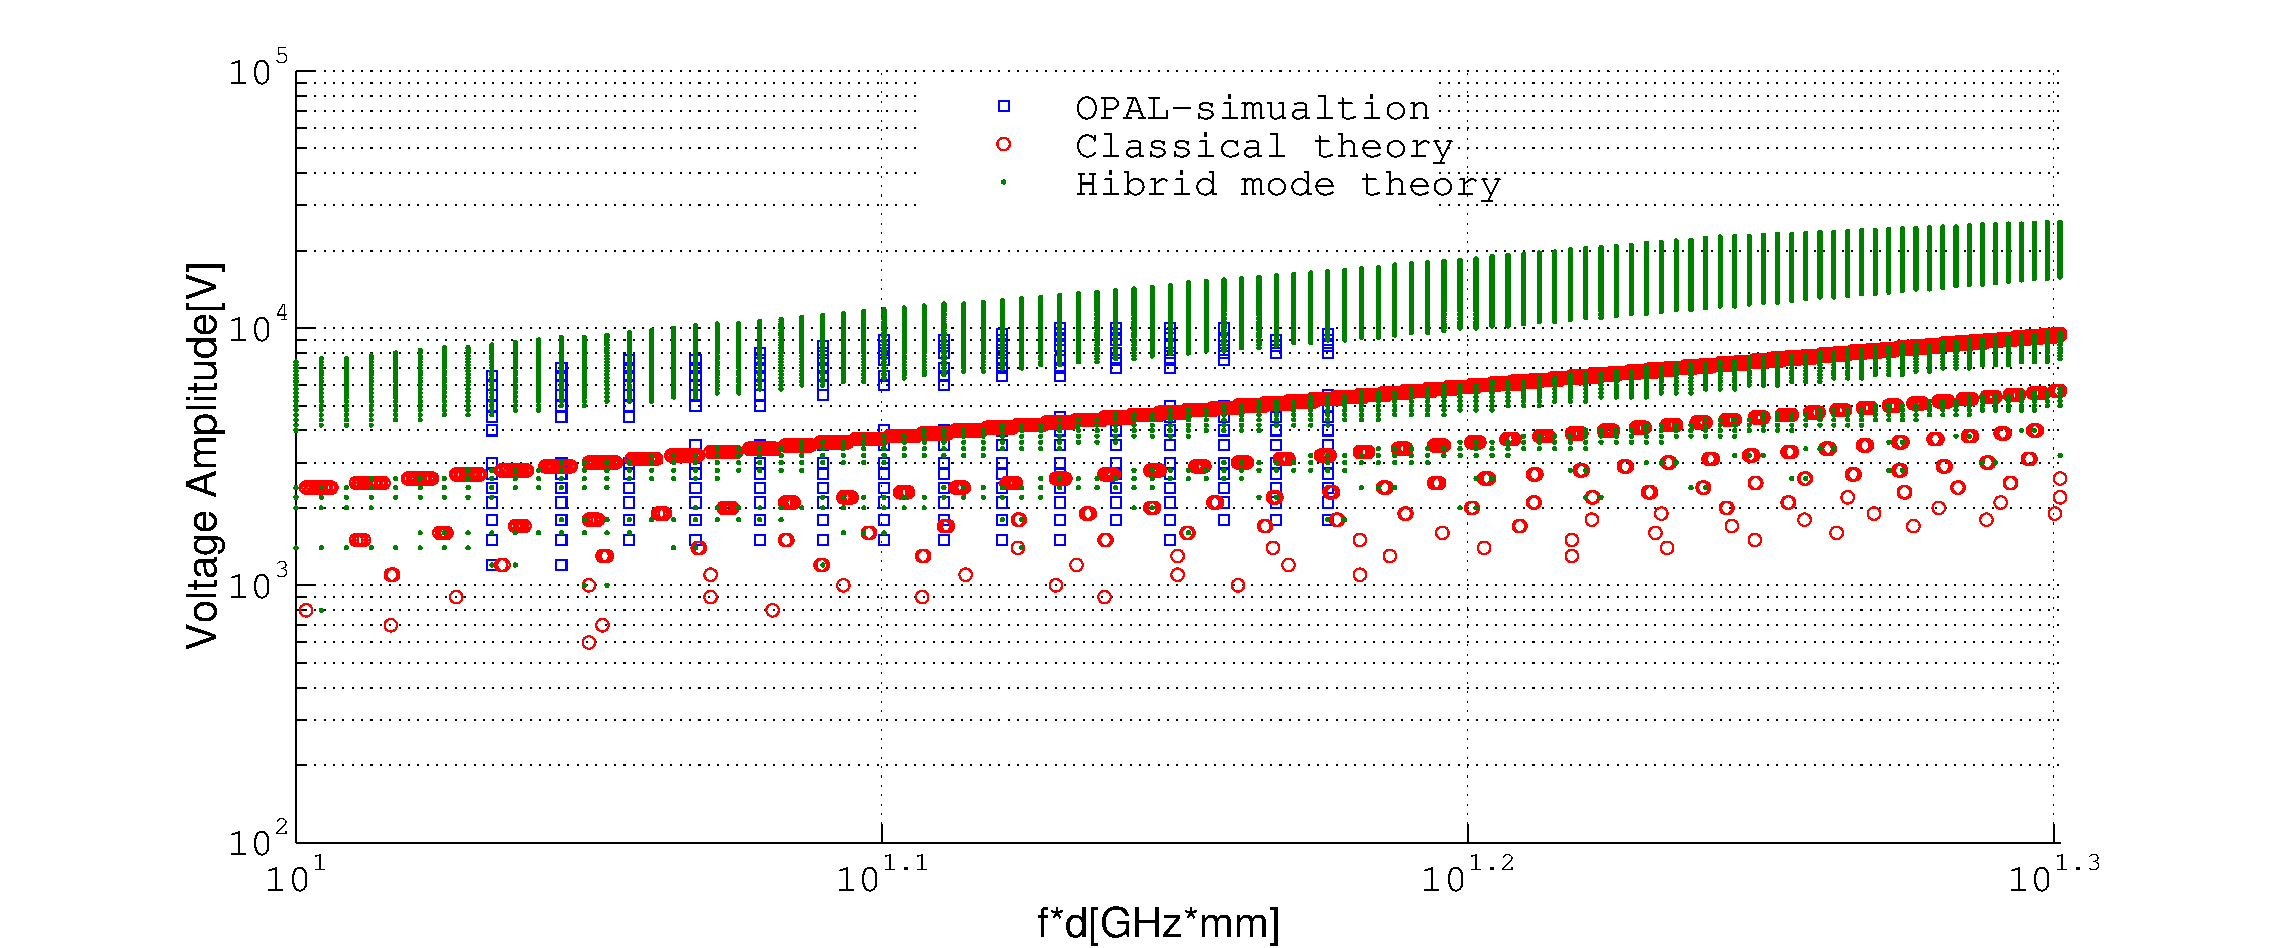
\includegraphics[width=1.0\textwidth]{benchmark2.pdf}
%/Users/adelmann/svnwork/adelmann/papers/figures/Latex-Figures/Incident.tikz
\end{center}
%\caption{Line segment-triangle intersection()\label{fig:L-T}}
\end{figure}
\begin{itemize}
\item Missing the single side impact which also plays an important role in multiplication
\end{itemize}
\end{frame}
\begin{frame}[allowframebreaks]
\frametitle{Non-stationary Multipacting Theory}
\begin{columns}
\begin{column}[t]{3cm}
\begin{figure}[H]
\begin{center}
\scalebox{0.5}{
\begin{tikzpicture}
\usetikzlibrary{arrows}
\draw [<->,thick] (0,0.8) node (zaxis) [above] {$\mathbf{z}$}
        |- (0.8,0) node (yaxis) [right] {$\mathbf{y}$};
\draw [->,thick] (0,0) -- (-0.5656,-0.5656) node (xaxis) [above] {$\mathbf{x}$};

\draw (-3.5,-1) -- (2.5,-1);
\draw (2.5,-1) -- (5,3);
\draw (0.5,3) -- (5,3);
\draw (-3.5,-1) -- (0.5,3);
\draw [<-] (-3.5,-1.05) -- (-3.5,-2.1) node (d) [left,below] {$\mathbf{d}$};
\draw [<-] (-3.5,-3.75) -- (-3.5,-2.7);
\draw (-3.5,-3.8) -- (2.5,-3.8);
\draw (2.5,-3.8) -- (4.5,-0.5);
\draw (-0.0,-0.5) -- (4.5,-0.5);
\draw (-3.5,-3.8) -- (0.0,-0.5);


\path[draw=black] (3.3,0.5) circle (2pt);
%\node[above=7pt,left=2pt] (I) at (0.5,0.5) {};
\path[draw=black,thick] (5.5,-1) circle (0.4);
\draw [] (3.3,0.5) arc (90:37:2.9);
\path[draw=black] (3.3,-2.5) circle (2pt);
\draw [] (3.3,-2.5) arc (-90:-34:2.6);
\draw [thick] (5.1,-1) sin (5.3,-0.9) cos (5.5,-1) sin (5.7,-1.1) cos (5.9,-1) sin (5.9,-1);
\node[above=7pt,right=12pt] (I) at (5.5,-1) {$\vec{E}=-\mathbf{\hat{z}}\frac{V_0}{d} \sin \omega t$};
\end{tikzpicture}
}

\end{center}
%\caption{Line segment-triangle intersection()\label{fig:L-T}}
\end{figure}
\end{column}
\begin{column}[t]{6cm}
\begin{itemize}
\item Parallel Plate (PP): \cite{NS}
\begin{align}
\frac{d^2z}{dt^2} &= -\frac{e}{m} E_0\sin\omega t \nonumber
\\
&= - \frac{e}{m}\frac{V_0}{d}\sin\omega t \label{scalar}
\end{align}
\item Random nature of emission energy(velocity): random impact phase, energy \ldots
\end{itemize}
\end{column}
\end{columns}
\end{frame}
\begin{frame}
\frametitle{Non-stationary Multipacting Theory(2)}
\begin{itemize}
\item Integrating equation \eqref{scalar} w.r.t variable $t$, and using initial conditions $\displaystyle \frac{dz}{dt}|_{t=t_0}=v_{0}$, $z|_{t=t_0}=0$, normalized variables:  $v_{\omega}=eV_0/m\omega d $, $\lambda=\omega d/v_{\omega}$, $u=v_{0}/v_{\omega}$, $\omega t_0=\varphi_0$, $\omega t=\varphi$
\begin{align}
z&=-\frac{d}{\lambda}\sin\omega t+\frac{d}{\lambda}(u+\cos\varphi_0)\omega t
\nonumber \\
&+\frac{d}{\lambda}\sin\varphi_0-\frac{d}{\lambda}(u+\cos\varphi_0)\varphi_0.\label{po}
\end{align}
\item if we define $\xi=\omega z/v_{\omega}$ and $\tau=\varphi-\varphi_0$ in consequence equation \eqref{po} can be rewritten by using this new variable as:
\begin{equation}
\xi(\varphi,\varphi_0,u) = (u+\cos \varphi_0)\tau+\sin \varphi_0 - \sin (\varphi_0+\tau).\label{nposition}
\end{equation}
\end{itemize}
\end{frame}
\begin{frame}
\frametitle{Non-stationary Multipacting Theory(3)}
\begin{columns}
\begin{column}[t]{7cm}
\begin{figure}[H]
\begin{center}
\scalebox{0.6}{
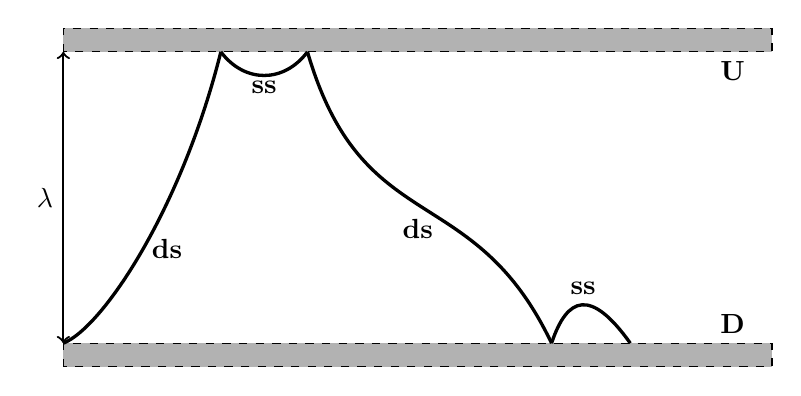
\begin{tikzpicture}
\usetikzlibrary{arrows}
\draw[fill=gray!60,dashed] (-3,0) rectangle (6,0.3);
\draw[fill=gray!60,dashed] (-3,-4) rectangle (6,-3.7);
\draw[very thick] (-3,-3.7) .. controls (-2.5,-3.5) and (-1.5,-2) .. (-1,0);
\draw[very thick] (-1,0) .. controls (-0.7,-0.4) and (-0.2,-0.4) .. (0.1,0);
\draw[very thick] (0.1,0) .. controls (0.8,-2.4) and (2.2,-1.6) .. (3.2,-3.7);
\draw[very thick] (3.2,-3.7) .. controls (3.4,-3.1) and (3.7,-3.0) .. (4.2,-3.7);
\draw (5.5,-3.7) node (d) [above] {$\mathbf{D}$};
\draw (5.5,0) node (u) [below] {$\mathbf{U}$};
\draw (-2.0,-2.5) node (ds1) [right] {$\mathbf{ds}$};
\draw (-0.45,-0.25) node (ss1) [below] {$\mathbf{ss}$};
\draw (1.5,-2) node (ds2) [below] {$\mathbf{ds}$};
\draw (3.6,-3.2) node (ss2) [above] {$\mathbf{ss}$};
%\draw [dashed,thick] (0,0.8) node (zaxis) [above] {$\mathbf{z}$}
%        |- (0.8,0) node (yaxis) [right] {$\mathbf{y}$};
\draw [<-,thick] (-3.,-3.7) -- (-3,-1.85) node (d) [left] {$\mathbf{\lambda}$};
\draw [<-,thick] (-3,0) -- (-3,-1.85);
\end{tikzpicture}
}
\end{center}
%\caption{Line segment-triangle intersection()\label{fig:L-T}}
\end{figure}
\end{column}
\begin{column}[t]{5cm}
\begin{itemize}
\item There double-side(ds) and single-side(ss) impacting exist
\item Correspond to $\xi(\varphi,\varphi_0,u)=\lambda$ and $\xi(\varphi,\varphi_0,u)=0$ in equation \eqref{nposition} 
\item More complete description of multipacting in PP
\end{itemize}
\end{column}
\end{columns}
\end{frame}
\begin{frame}
\frametitle{Non-stationary Multipacting Theory(4)}
\begin{itemize}
\item As the initial velocity $u$ of emitted particles is a random variable, the solution of equation \eqref{nposition} w.r.t the time $\tau$ that particles hit the plates is also a random variable 
\item As long as we know the probability density function (PDF) of the initial velocity $u$, which usually is a thermal distribution, then the PDF of time $\tau$ can be derived according to the rule of change of variable in probability theory
\end{itemize}
\end{frame}
\begin{frame}
\frametitle{Non-stationary Multipacting Theory(5)}
\begin{itemize}
\item The electron emission rates and impact rates in each plate can be described by the PDF of the time $\tau$, at which particles hit the plates, and the secondary emission yield coefficient w.r.t $\tau$ and $u$
\item The particle number can be obtained by integrating the emission rates and impact rates w.r.t time (details please see the appendix of this talk and also Ref \cite{NS} )
\end{itemize}
\end{frame}
\subsection{Goal of Our Work}
\begin{frame}
\begin{itemize}
\item Extend OPAL with complex geometry handling capabilities (geometry format compatible with the FEM field solver FEMAXX)
\item Add dark current and multipacting simulation capabilities to OPAL to handle complex RF structures with arbitrary geometries
\item Post processing and visualization 
\item Report(s) and paper(s)  
\end{itemize}
\end{frame}
\section{Geometry handling and surface physics models}
\subsection{Geometry Handling}
\begin{frame}
\frametitle{3D Geometry Handling Capability for OPAL}
\begin{itemize}
\item Read in surface mesh generated by Heronion or GMSH in FEMAXX format (future in H5HUT/H5FED)
\item Triangle-line segment intersection test and boundary box strategy based collision test
\item We can handle arbitrary structure as long as it is closed 
\end{itemize}
\end{frame}
\begin{frame}[allowframebreaks]
\frametitle{3D Geometry model in OPAL}
\begin{itemize}
\item Triangulated surface representation of geometry
\begin{columns}
\begin{column}[t]{6cm}
\begin{figure}
\begin{center}
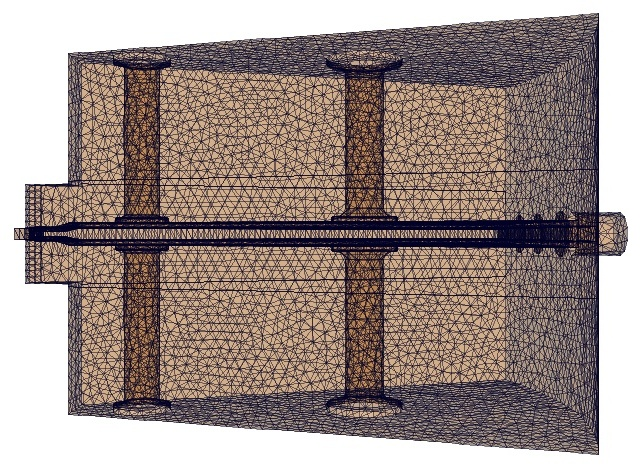
\includegraphics[width=0.9\textwidth]{cyclotron_cavity_mesh.jpg}
%
\scalebox{0.7}{
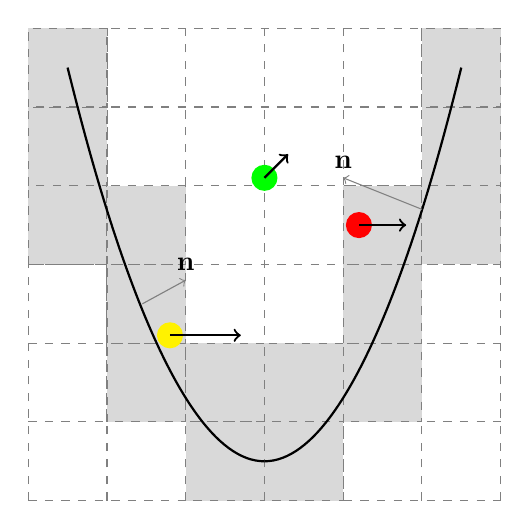
\begin{tikzpicture}
\draw[step=1cm,gray,dashed] (-3,0) grid (3,6);
\draw[step=1cm,gray,dashed,fill=gray!30] (-3,3) rectangle (-2,4); 
\draw[step=1cm,gray,dashed,fill=gray!30] (-2,1) rectangle (-1,2); 
\draw[step=1cm,gray,dashed,fill=gray!30] (-2,2) rectangle (-1,3); 
\draw[step=1cm,gray,dashed,fill=gray!30] (-2,3) rectangle (-1,4);
\draw[step=1cm,gray,dashed,fill=gray!30] (-1,1) rectangle (0,2);
\draw[step=1cm,gray,dashed,fill=gray!30] (-1,0) rectangle (0,1);
\draw[step=1cm,gray,dashed,fill=gray!30] (0,0) rectangle (1,1);
\draw[step=1cm,gray,dashed,fill=gray!30] (0,1) rectangle (1,2);
\draw[step=1cm,gray,dashed,fill=gray!30] (1,1) rectangle (2,2);
\draw[step=1cm,gray,dashed,fill=gray!30] (1,2) rectangle (2,3); 
\draw[step=1cm,gray,dashed,fill=gray!30] (1,3) rectangle (2,4);
\draw[step=1cm,gray,dashed,fill=gray!30] (2,3) rectangle (3,4);
\draw[step=1cm,gray,dashed,fill=gray!30] (-3,4) rectangle (-2,5);
\draw[step=1cm,gray,dashed,fill=gray!30] (-3,5) rectangle (-2,6);
\draw[step=1cm,gray,dashed,fill=gray!30] (2,4) rectangle (3,5);
\draw[step=1cm,gray,dashed,fill=gray!30] (2,5) rectangle (3,6);   
\draw[black, thick] (0.,0.5) parabola  ( 2.5,5.5); 
\draw[black, thick] (0.,0.5) parabola  ( -2.5,5.5);
\draw [->,gray] (-1.55,2.5) -- (-1,2.8);
\node[above] (n) at (-1,2.8) {$\vec{n}$};
\draw [<-,gray] (1.0,4.1) -- (2,3.7);
\node[above] (n) at (1,4.1) {$\vec{n}$};
%\tikz[label distance=4mm]
\draw (-1.2,2.1) node[circle,fill=yellow]{};
\draw [->,thick] (-1.2,2.1) -- (-0.3,2.1);
\draw (0,4.1) node[circle,fill=green]{};
\draw [->,thick] (0,4.1) -- (0.3,4.4);
\draw (1.2,3.5) node[circle,fill=red]{};
\draw [<-,thick] (1.8,3.5) -- (1.2,3.5);
\end{tikzpicture}
}
\end{center}
%\caption{Line segment-triangle intersection()\label{fig:L-T}}
\end{figure}
\end{column}
\begin{column}[t]{6cm}
\begin{figure}
\begin{center}
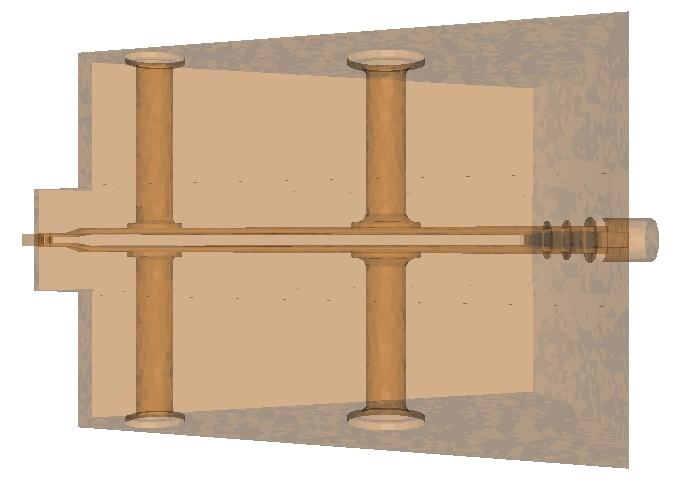
\includegraphics[width=1.0\textwidth]{cyclotron_cavitry.jpg}
\end{center}
%\caption{Line segment-triangle intersection()\label{fig:L-T}}
\end{figure}
\end{column} 
\end{columns}

\begin{figure}
\begin{center}
\scalebox{0.7}{
\begin{tikzpicture}
\usetikzlibrary{arrows}
\draw [->,black,-latex] (-1.5,0) -- (1.5,0);
\draw [->,black,-latex] (-1.5,0) -- (-1.5,2);
\draw (1.5,0) -- (0.0,2);
\draw  [<-,black,latex-](0.0,2) -- (-1.5,0.0);
\draw [->,black,-latex,dashed] (-1.5,0) -- (0.5,0.5);
\node[below] (w) at (-0.15,0.5) {$\vec{w}$};
\draw[dashed] (0.5,0.5) -- (-1.18,0.5);
\draw[dashed] (0.5,0.5) -- (0.01,0.0);
\node[above] (ti) at (-1.18,0.5) {$t_i$};
\node[below] (si) at (0.01,0.0) {$s_i$};
\node[above] (t0) at (-1.7,0.) {$\mathbf{t_0}$};
\node[right] (t1) at (1.5,0) {$\mathbf{t_1}$};
\node[above] (t2) at (0.0,2.0) {$\mathbf{t_2}$};
\node[above] (n) at (-1.5,2) {$\vec{n}$};
\node[above] (v) at (-0.5,1.5) {$\vec{v}$};
\node[below] (u) at (1.2,0.0) {$\vec{u}$};
\path[draw=black,fill=black] (0.0,2.0) circle (2pt);
\path[draw=black,fill=black] (1.5,0.0) circle (2pt);
\path[draw=black,fill=black] (-1.5,0.0) circle (2pt);
\draw (-3.5,-1) -- (2.5,-1);
\draw (2.5,-1) -- (5,3);
\draw (0,3) -- (5,3);
\draw (-3.5,-1) -- (0,3);
\draw (0.5,0.5) -- (1.6,5);
\path[draw=black] (0.5,0.5) circle (2pt);
\node[above] (I) at (0.5,0.5) {$\mathbf{I}$};
\node[right] (x0) at (1.6,5) {$\mathbf{x_0}$};
\draw[dashed] (0.5,0.5) -- (-0.1,-1.9);
\node[right] (x1) at (0.0,-1.9) {$\mathbf{x_1}$};
\node[right] (ri) at (1,2.5) {$r_i$};
\path[draw=black,fill=black] (-0.1,-1.9) circle (2pt);
\path[draw=black,fill=black] (1.6,5) circle (2pt);
\end{tikzpicture}
}
\end{center}
%\caption{Line segment-triangle intersection()\label{fig:L-T}}
\end{figure}
\item Line segment-Triangle intersection test 
\begin{figure}
\begin{center}

\scalebox{0.7}{
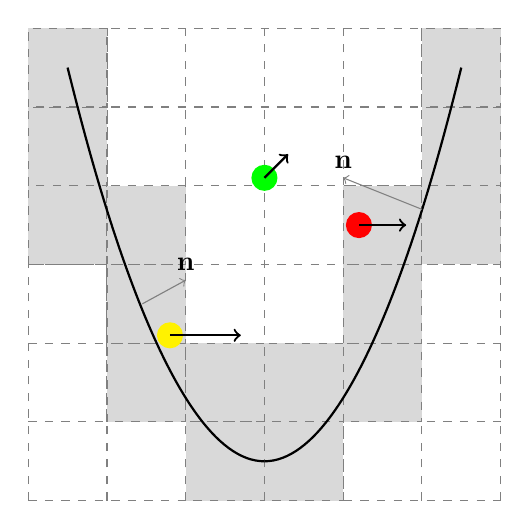
\begin{tikzpicture}
\draw[step=1cm,gray,dashed] (-3,0) grid (3,6);
\draw[step=1cm,gray,dashed,fill=gray!30] (-3,3) rectangle (-2,4); 
\draw[step=1cm,gray,dashed,fill=gray!30] (-2,1) rectangle (-1,2); 
\draw[step=1cm,gray,dashed,fill=gray!30] (-2,2) rectangle (-1,3); 
\draw[step=1cm,gray,dashed,fill=gray!30] (-2,3) rectangle (-1,4);
\draw[step=1cm,gray,dashed,fill=gray!30] (-1,1) rectangle (0,2);
\draw[step=1cm,gray,dashed,fill=gray!30] (-1,0) rectangle (0,1);
\draw[step=1cm,gray,dashed,fill=gray!30] (0,0) rectangle (1,1);
\draw[step=1cm,gray,dashed,fill=gray!30] (0,1) rectangle (1,2);
\draw[step=1cm,gray,dashed,fill=gray!30] (1,1) rectangle (2,2);
\draw[step=1cm,gray,dashed,fill=gray!30] (1,2) rectangle (2,3); 
\draw[step=1cm,gray,dashed,fill=gray!30] (1,3) rectangle (2,4);
\draw[step=1cm,gray,dashed,fill=gray!30] (2,3) rectangle (3,4);
\draw[step=1cm,gray,dashed,fill=gray!30] (-3,4) rectangle (-2,5);
\draw[step=1cm,gray,dashed,fill=gray!30] (-3,5) rectangle (-2,6);
\draw[step=1cm,gray,dashed,fill=gray!30] (2,4) rectangle (3,5);
\draw[step=1cm,gray,dashed,fill=gray!30] (2,5) rectangle (3,6);   
\draw[black, thick] (0.,0.5) parabola  ( 2.5,5.5); 
\draw[black, thick] (0.,0.5) parabola  ( -2.5,5.5);
\draw [->,gray] (-1.55,2.5) -- (-1,2.8);
\node[above] (n) at (-1,2.8) {$\vec{n}$};
\draw [<-,gray] (1.0,4.1) -- (2,3.7);
\node[above] (n) at (1,4.1) {$\vec{n}$};
%\tikz[label distance=4mm]
\draw (-1.2,2.1) node[circle,fill=yellow]{};
\draw [->,thick] (-1.2,2.1) -- (-0.3,2.1);
\draw (0,4.1) node[circle,fill=green]{};
\draw [->,thick] (0,4.1) -- (0.3,4.4);
\draw (1.2,3.5) node[circle,fill=red]{};
\draw [<-,thick] (1.8,3.5) -- (1.2,3.5);
\end{tikzpicture}
}
\end{center}
%\caption{Line segment-triangle intersection()\label{fig:L-T}}
\end{figure}
\item Boundary bounding box to speedup the collision tests
\end{itemize}
\end{frame}
\subsection{Surface Physics Models}
\begin{frame}
\frametitle{Field Emission Model}
\begin{itemize}
\item Fowler-Nordheim formula introduced by \cite{FN} and implemented for dark current simulation by \cite{DE}: $J(\mathbf{r},t) = \frac{A(\beta E)^2}{\varphi t(y)^2}\exp{(\frac{-B v(y)\varphi^{3/2}}{\beta E})}$
\item Child-Langmuir law: space charge limited current
\begin{align*}
J(\mathbf{r},t) & =\frac{4\varepsilon_0}{9}\sqrt{2\frac{e}{m}}(\frac{V^{3/2}}{d^2})\\
 & =\frac{4\varepsilon_0}{9}\sqrt{2\frac{e}{m}}(\frac{E^{3/2}}{d^{1/2}})
\end{align*}
\end{itemize}
\end{frame}
\begin{frame}
\frametitle{Secondary Emission Model by Furman \& Pivi}
\begin{itemize}
\item Mathematically self-consistent
\item Phenomenological- don't involve secondary physics but fit the data
\item A number of parameters to fit the measured SEY data
\item Built-in SEY data for copper and stainless steel
\item Monte Carlo technique has been used
\item Detailed description on algorithms see \cite{SE}
\end{itemize}
\end{frame}
\begin{frame}[allowframebreaks]
\frametitle{Secondary Emission Model: Vaughan's Formula}
\begin{itemize}
\item For material other than copper and stainless steel or material with different SEY curve from the built-in SEY curve in Furman-Pivi's model, Vaughan's model has less parameters than Furman-Pivi's model thus relatively easier to be adjusted to fit the new SEY curve
\item Vaughan's formula:
\begin{subequations}
\label{allequations}
\begin{eqnarray}
    \delta(E,\theta)&=&\delta_{max}(\theta)\cdot (v e^{1-v})^k,\ \text{for}\ v \le 3.6 \label{eq:VaughanA} 
\\
\delta(E,\theta)&=&\delta_{max}(\theta)\cdot 1.125/v^{0.35},\ \text{for}\ v > 3.6 \label{eq:VaughanB} 
\end{eqnarray}
\end{subequations}
where 
\begin{eqnarray*}
v=\frac{\displaystyle E-E_0}{\displaystyle E_{max}(\theta)-E_0},
\end{eqnarray*}
\begin{eqnarray*}
k=0.56,\ \ \text{for}\ v<1,
\end{eqnarray*}
\begin{eqnarray*}
k=0.25,\ \ \text{for}\ 1<v\le{3.6},
\end{eqnarray*}
\begin{eqnarray*}
\delta_{max}(\theta)=\delta_{max}(0)\cdot (1+k_{\theta}\theta^2/2\pi),
\end{eqnarray*}
\begin{eqnarray*}
E_{max}(\theta)=E_{max}(0)\cdot (1+k_E\theta^2/2\pi).
\end{eqnarray*}
\item User adjustable parameters: $E_{max}(0)$, $E_0$, $\delta_{max}(0)$, $\delta_{0}$, $k_{\theta}$ and $k_E$
\end{itemize}
\end{frame}
\section{Benchmark Results}
\subsection{Code to Code Benchmark of Furman-Pivi's model}
\begin{frame}
\frametitle{Benchmark Against the TxPhysics Library}
\begin{columns}
\begin{column}[t]{5.cm}
\begin{figure}[H]
\begin{center}
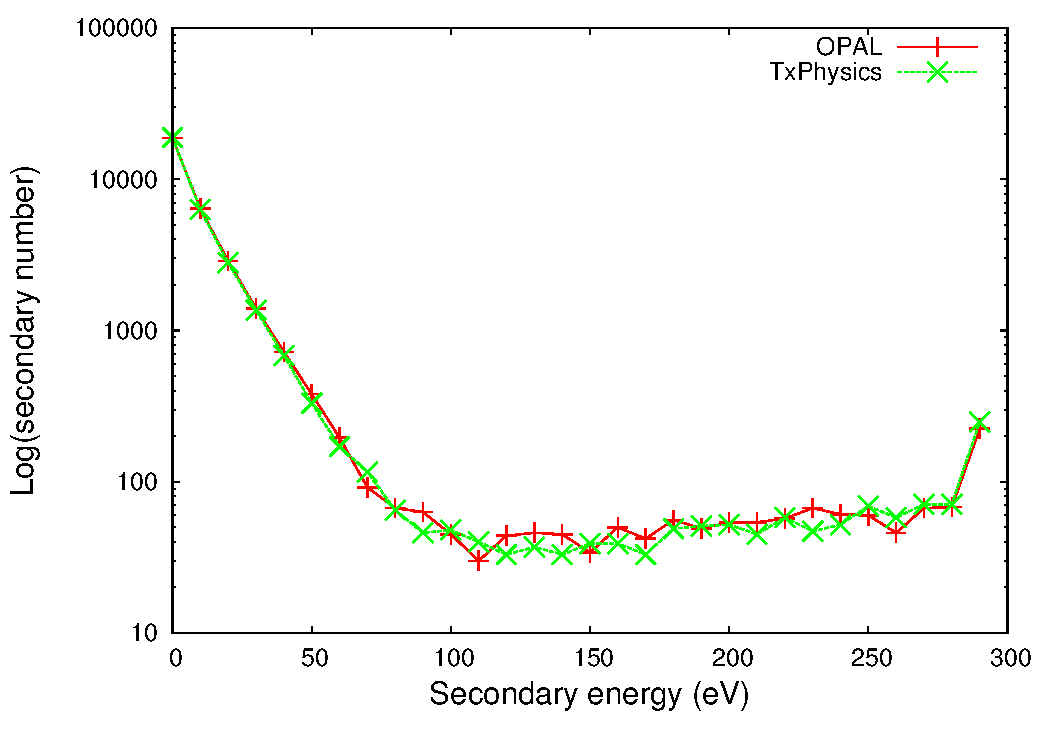
\includegraphics[width=1.2\textwidth]{code_comparison.pdf}
\end{center}
\end{figure}
\end{column}
\begin{column}[t]{5cm}
\begin{itemize}
\item Validate the implementation of Furman-Pivi's model
\item Logarithm of total secondary emission number (backscattered + re-diffused + true secondaries) vs. energy of emitted particles
\end{itemize}
\end{column}
\end{columns}
\end{frame} % to enforce entries in the table of contents
\subsection{BENCHMARK AGAINST NON-STATIONARY THEORY}
\begin{frame}
\frametitle{Why the Non-stationary Theory?}
\begin{itemize}
\item Only benchmarking the implementation of secondary emission model is not sufficient, the tracking process and non trivial geometry handling stuff also need to be benchmarked
\item Simple geometry
\begin{figure}[H]
\begin{center}
\scalebox{0.7}{
\scalebox{0.5}{
\begin{tikzpicture}
\usetikzlibrary{arrows}
\draw [<->,thick] (0,0.8) node (zaxis) [above] {$\mathbf{z}$}
        |- (0.8,0) node (yaxis) [right] {$\mathbf{y}$};
\draw [->,thick] (0,0) -- (-0.5656,-0.5656) node (xaxis) [above] {$\mathbf{x}$};

\draw (-3.5,-1) -- (2.5,-1);
\draw (2.5,-1) -- (5,3);
\draw (0.5,3) -- (5,3);
\draw (-3.5,-1) -- (0.5,3);
\draw [<-] (-3.5,-1.05) -- (-3.5,-2.1) node (d) [left,below] {$\mathbf{d}$};
\draw [<-] (-3.5,-3.75) -- (-3.5,-2.7);
\draw (-3.5,-3.8) -- (2.5,-3.8);
\draw (2.5,-3.8) -- (4.5,-0.5);
\draw (-0.0,-0.5) -- (4.5,-0.5);
\draw (-3.5,-3.8) -- (0.0,-0.5);


\path[draw=black] (3.3,0.5) circle (2pt);
%\node[above=7pt,left=2pt] (I) at (0.5,0.5) {};
\path[draw=black,thick] (5.5,-1) circle (0.4);
\draw [] (3.3,0.5) arc (90:37:2.9);
\path[draw=black] (3.3,-2.5) circle (2pt);
\draw [] (3.3,-2.5) arc (-90:-34:2.6);
\draw [thick] (5.1,-1) sin (5.3,-0.9) cos (5.5,-1) sin (5.7,-1.1) cos (5.9,-1) sin (5.9,-1);
\node[above=7pt,right=12pt] (I) at (5.5,-1) {$\vec{E}=-\mathbf{\hat{z}}\frac{V_0}{d} \sin \omega t$};
\end{tikzpicture}
}

}
\end{center}
%\caption{Line segment-triangle intersection()\label{fig:L-T}}
\end{figure}
\end{itemize}
\end{frame}  
\begin{frame}
\frametitle{First Case: None Severe Multiplication}
\begin{figure}[H]
\begin{center}
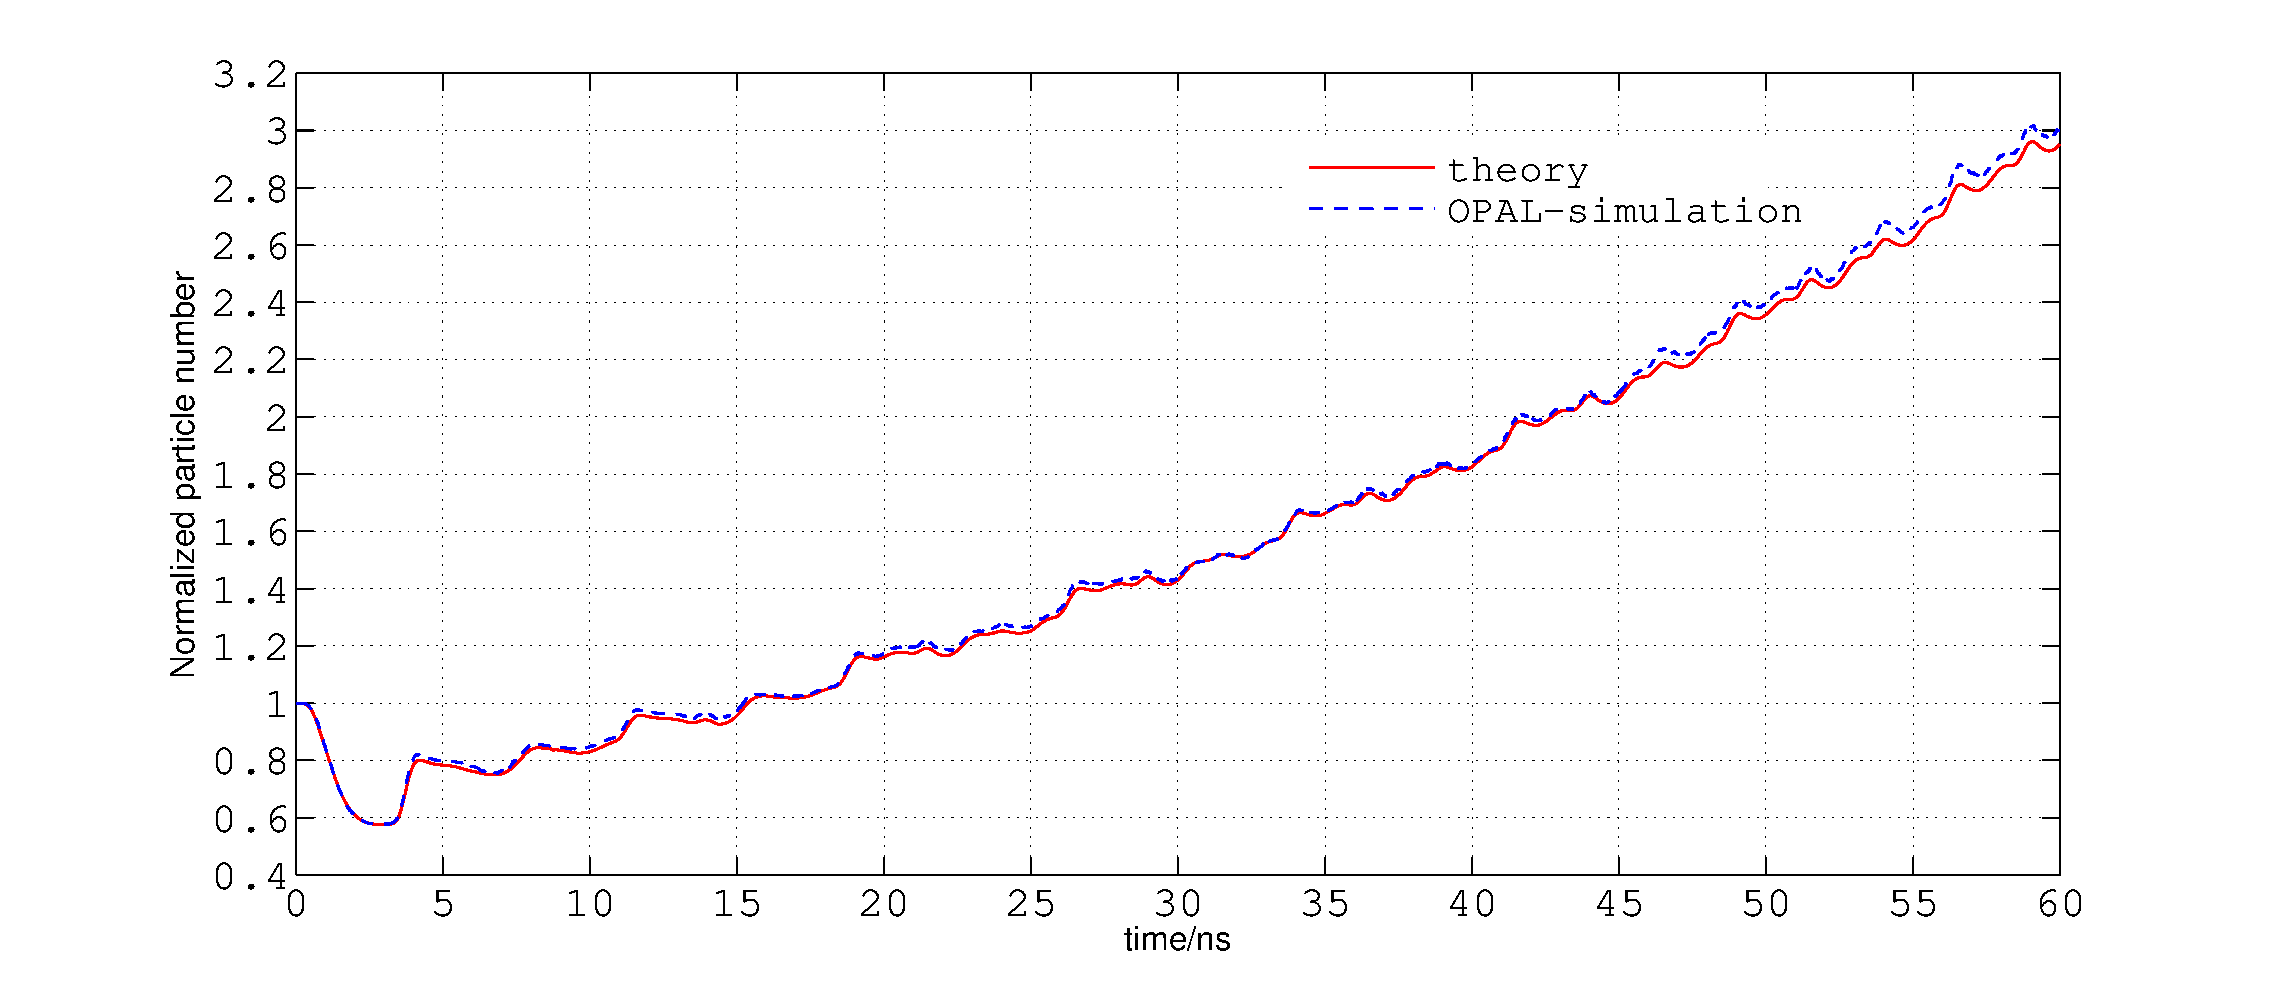
\includegraphics[width=1\textwidth]{match.pdf}
\end{center}
\end{figure}
\begin{itemize}
\item $f=200$MHz, $V_0=1200$V, $d=30$mm, Furman and Pivi's model and copper's SEY data
\end{itemize}
\end{frame} % to enforce entries in the table of contents
\begin{frame}
\frametitle{Real Number of Simulation Particles}
\begin{figure}[H]
\begin{center}
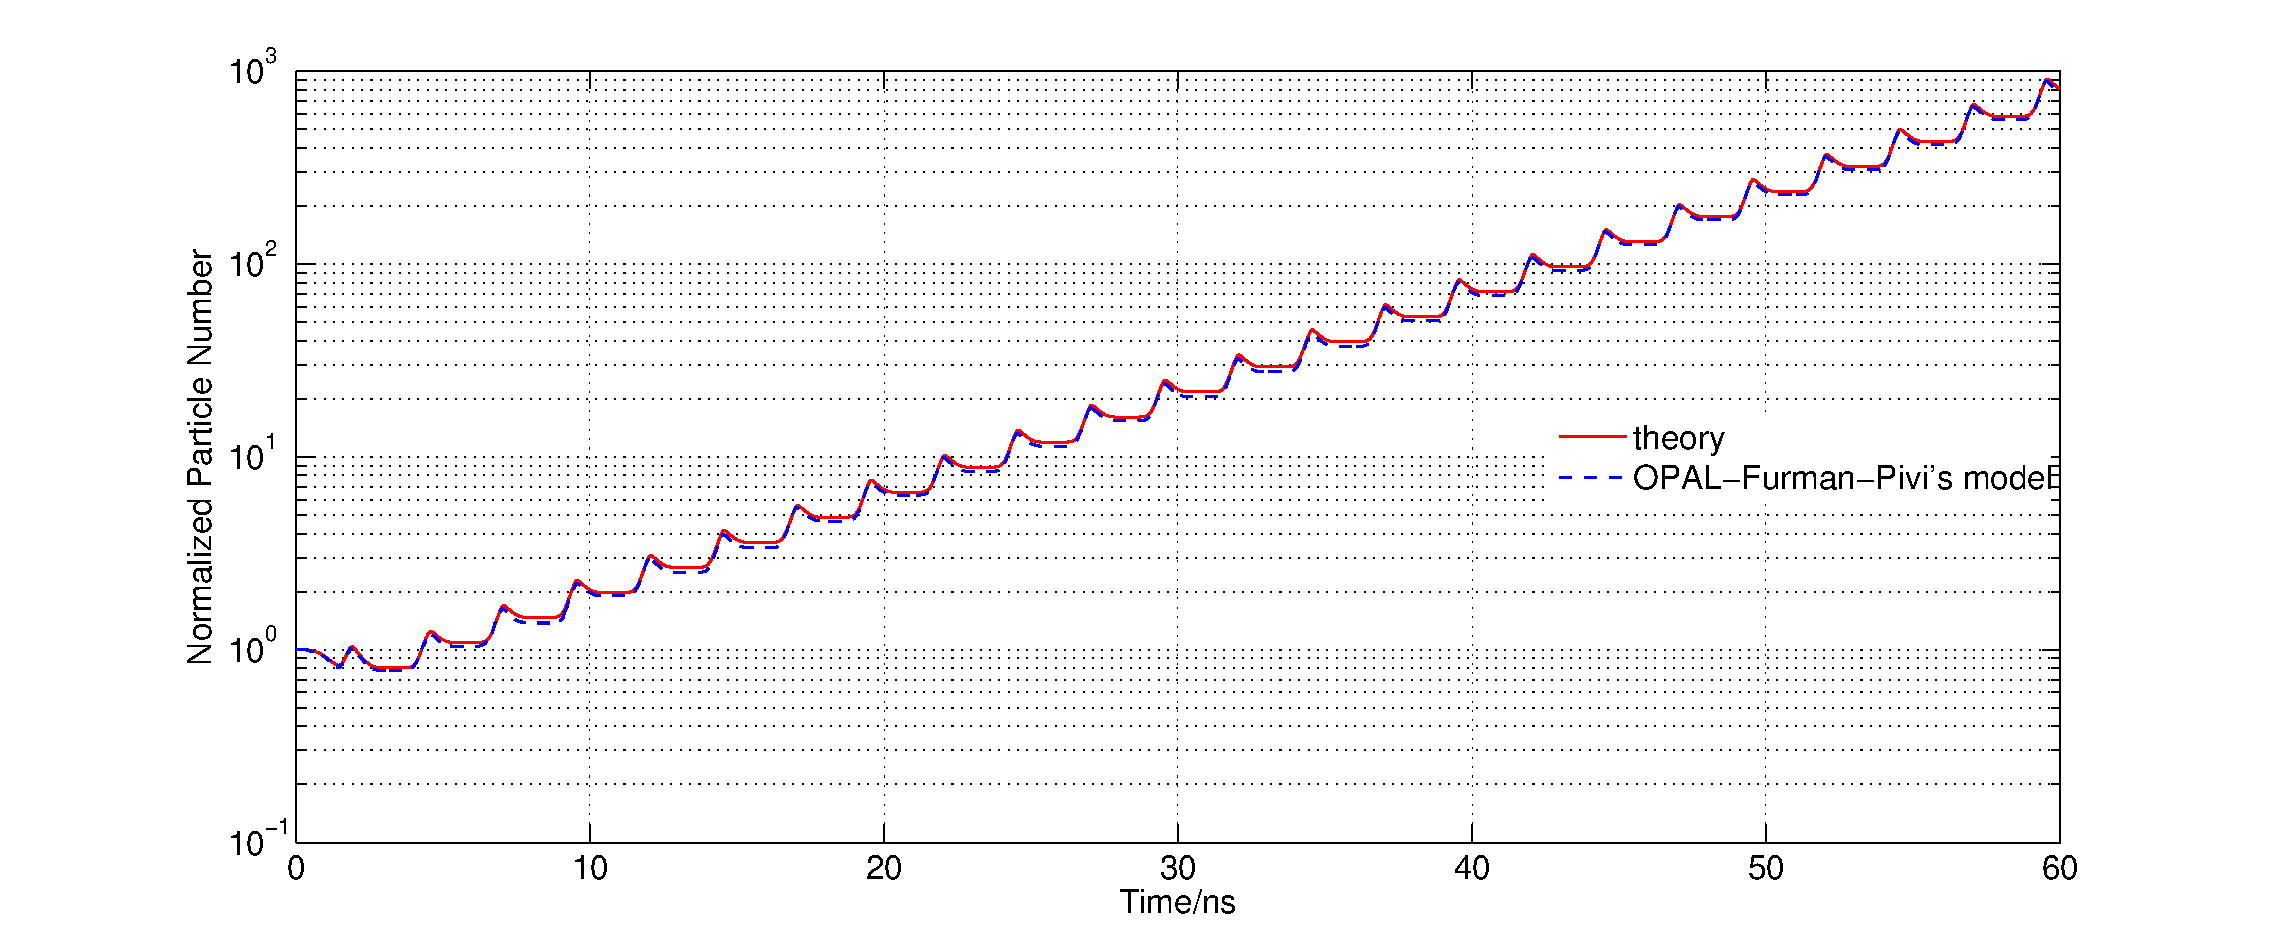
\includegraphics[width=1\textwidth]{copper_multi.pdf}
\end{center}
\end{figure}
\begin{itemize}
\item $f=200MHz$, $V_0=120V$, $d=5mm$, Furman and Pivi's model and copper's SEY data
\end{itemize}
\end{frame} % to enforce entries in the table of contents
\begin{frame}
\frametitle{Real Number of Simulation Particles}
\begin{figure}[H]
\begin{center}
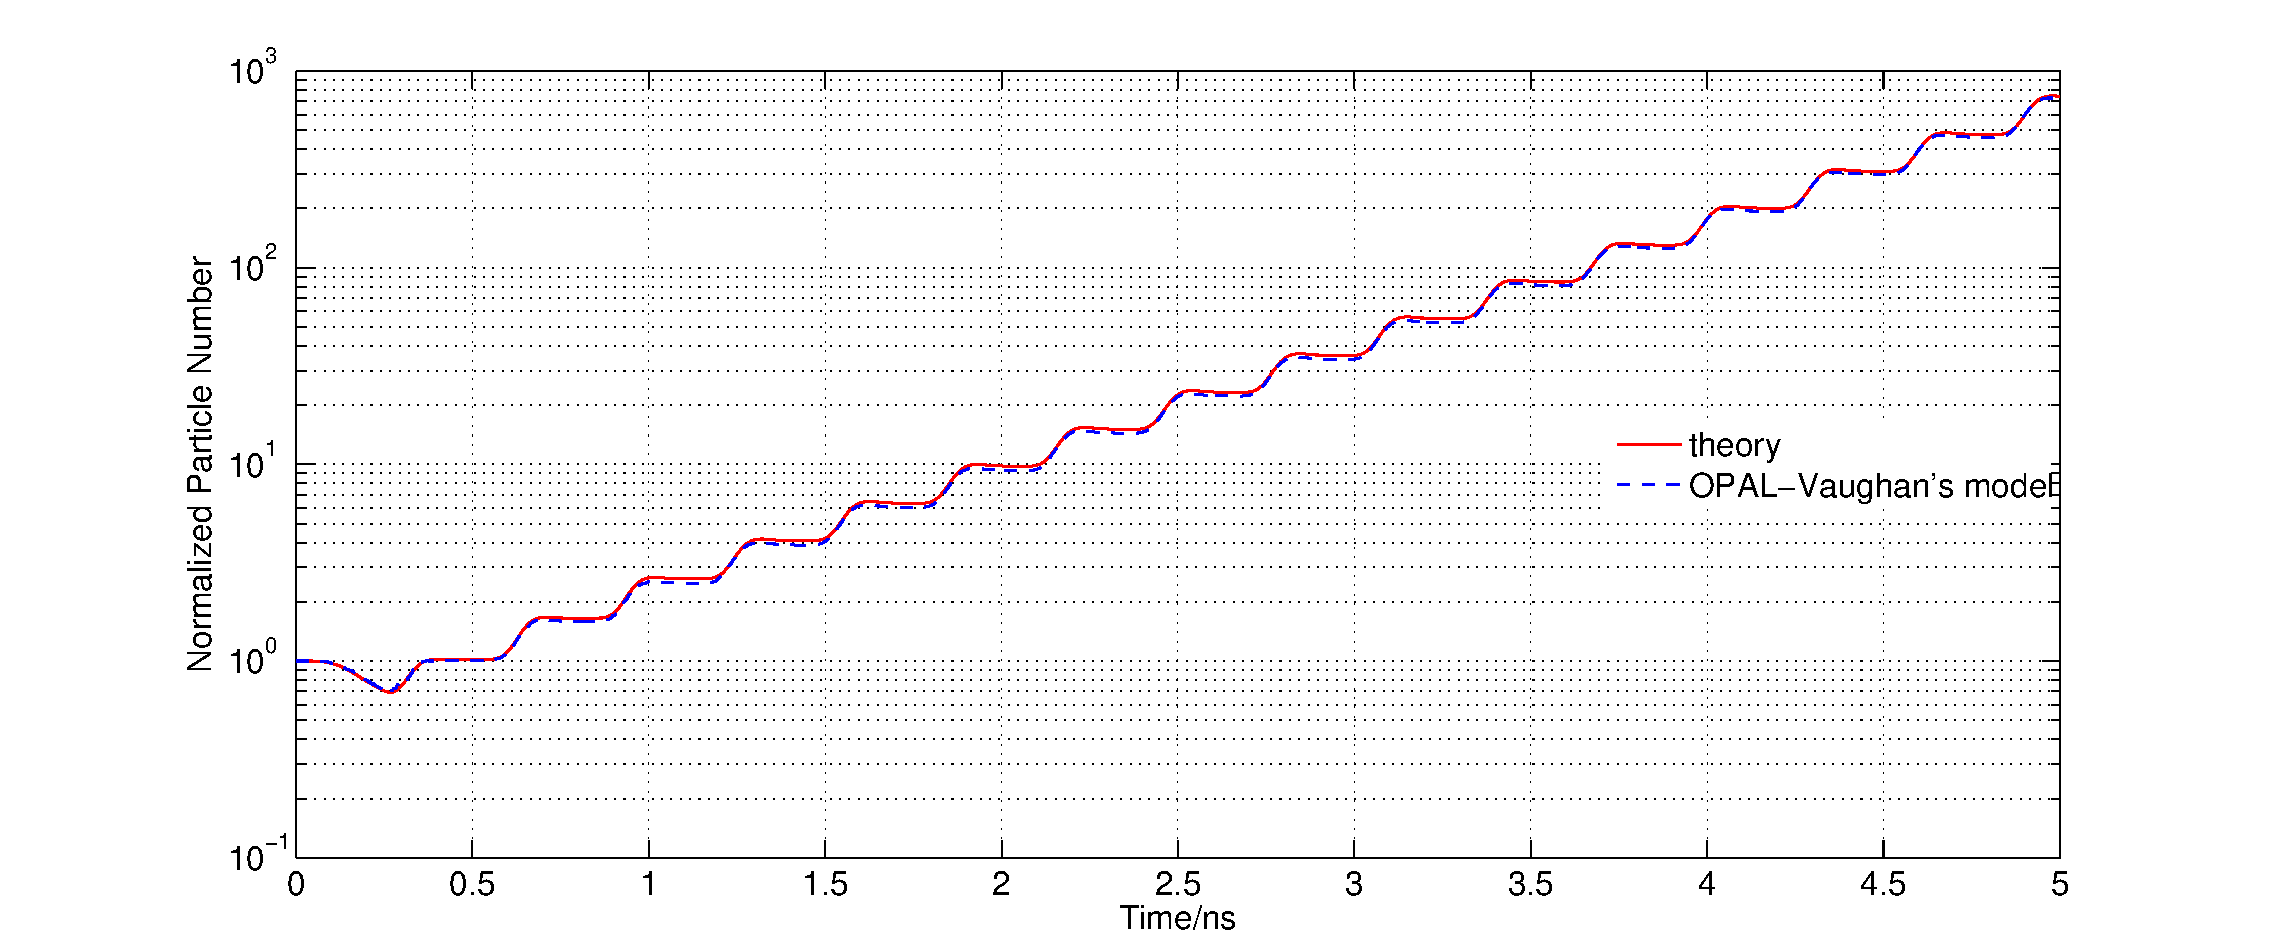
\includegraphics[width=1\textwidth]{silver_multi.pdf}
\end{center}
\end{figure}
\begin{itemize}
\item $f=1640MHz$, $V_0=120V$, $d=1mm$, using Vaughan's model and silver's SEY data
\end{itemize}
\end{frame} % to enforce entries in the table of contents
\begin{frame}
\frametitle{Real Number of Simulation Particles}
\begin{figure}[H]
\begin{center}
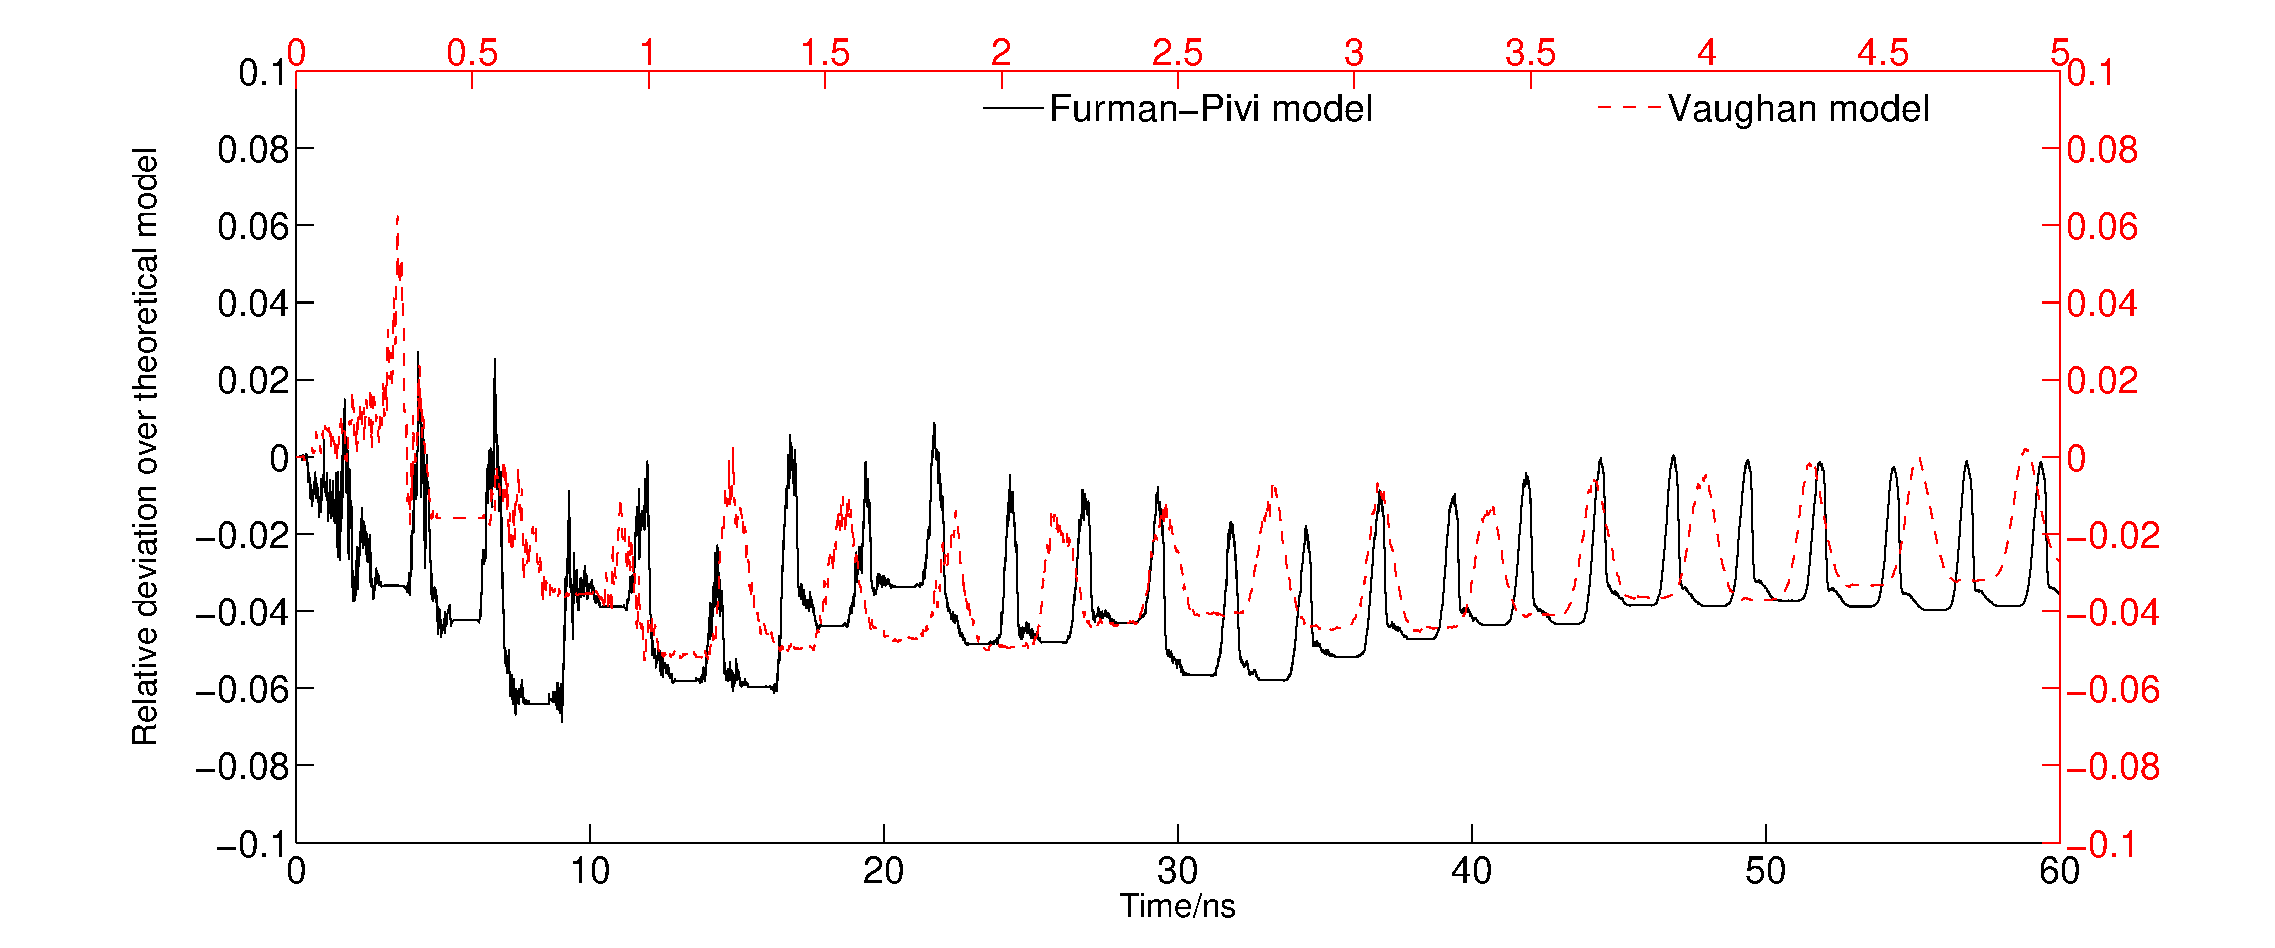
\includegraphics[width=1\textwidth]{models_comp.pdf}
\end{center}
\end{figure}
\begin{itemize}
\item Relative deviations of above simulation results over theoretical model predicted values
\end{itemize}
\end{frame} % to enforce entries in the table of contents
\begin{frame}[allowframebreaks]
\frametitle{Renormalized Simulation Particles}
\begin{figure}[H]
\begin{center}
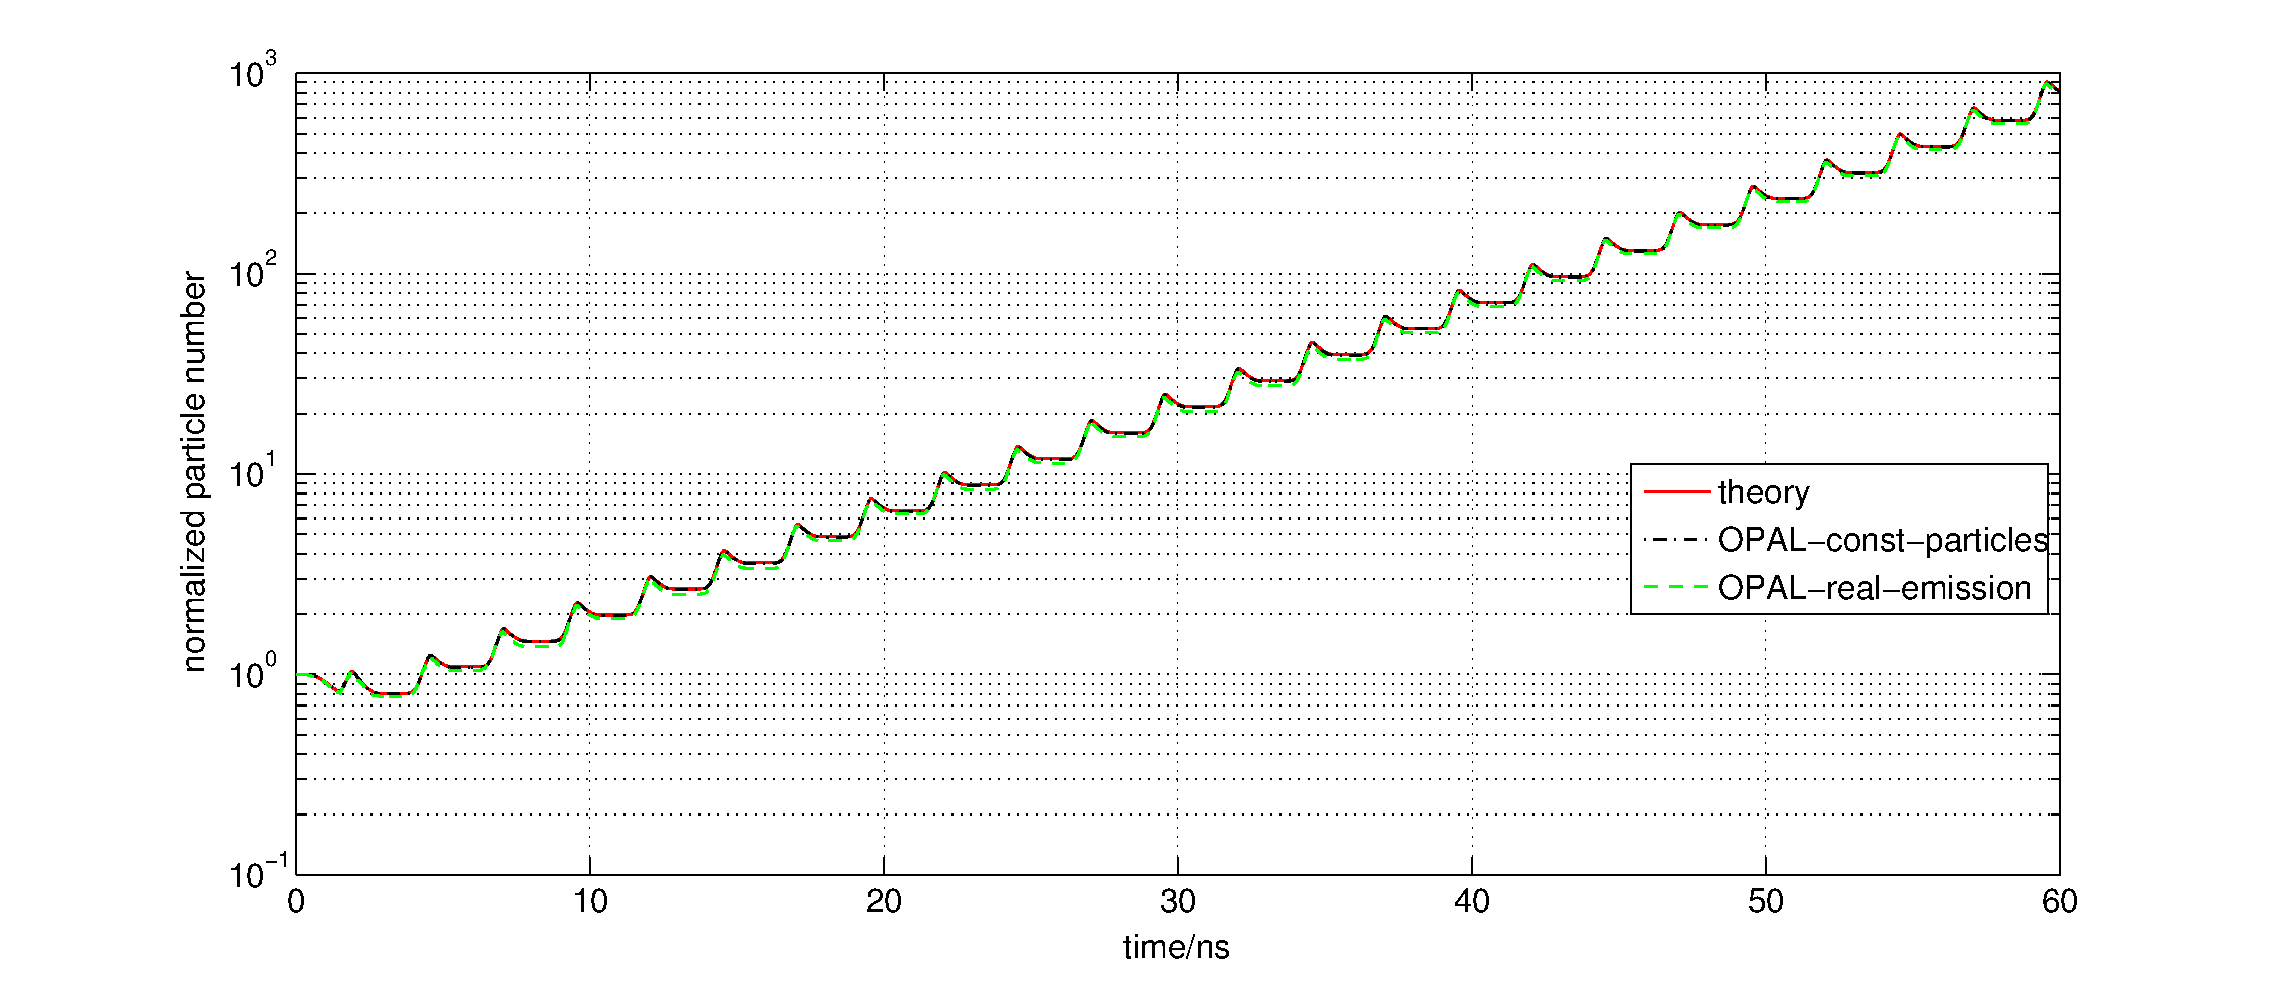
\includegraphics[width=0.95\textwidth]{const_particle_benchmark_FurmanPivi.pdf}
\end{center}
\end{figure}
\begin{itemize}
\item $f=200MHz$, $V_0=120V$, $d=5mm$, Furman-Pivi's model, copper and re-normalize to const simulation particle
\begin{figure}[H]
\begin{center}
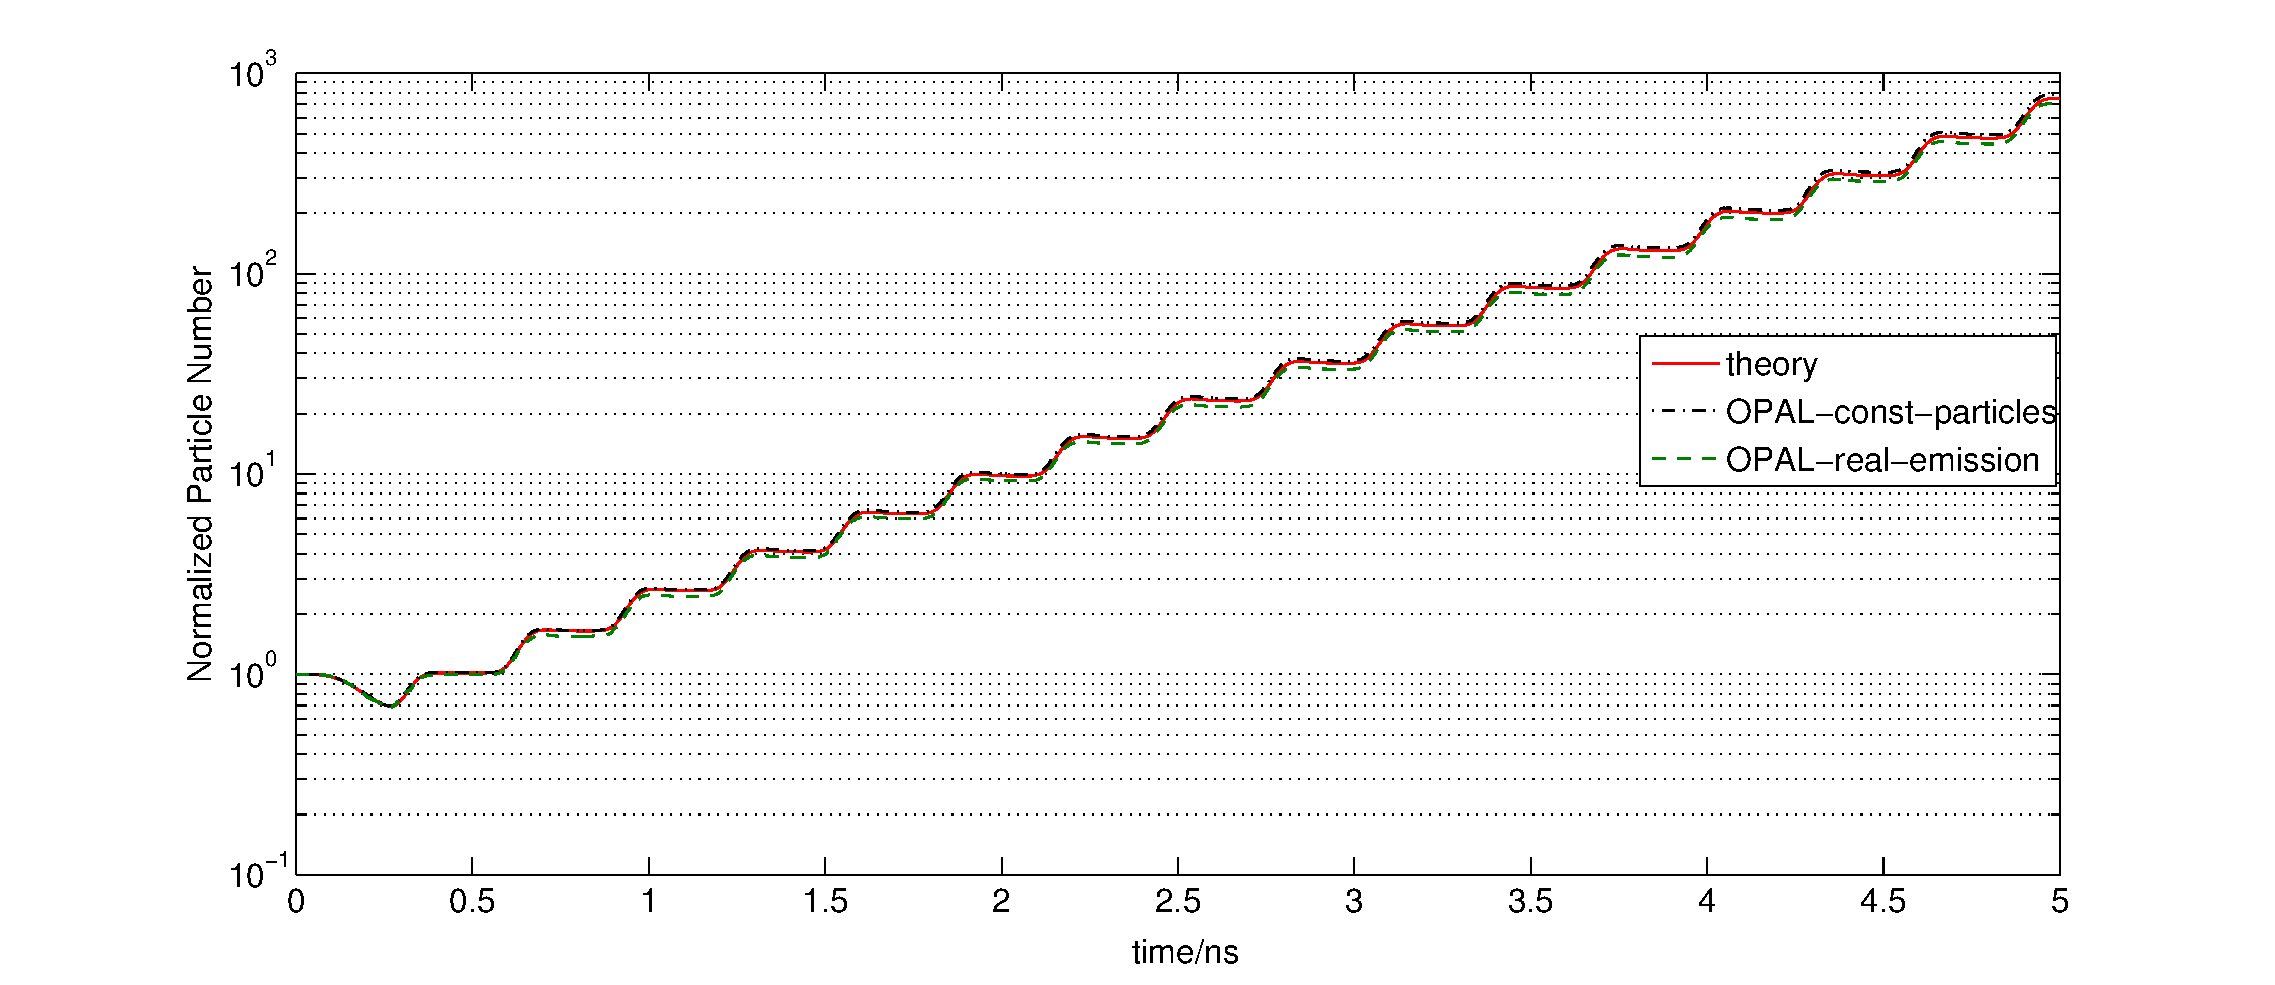
\includegraphics[width=0.95\textwidth]{const_particle_benchmark.pdf}
\end{center}
\end{figure}
\item $f=1640MHz$, $V_0=120V$, $d=1mm$, Vaughan's model, silver and re-normalize to const simulation particle
\begin{figure}[H]
\begin{center}
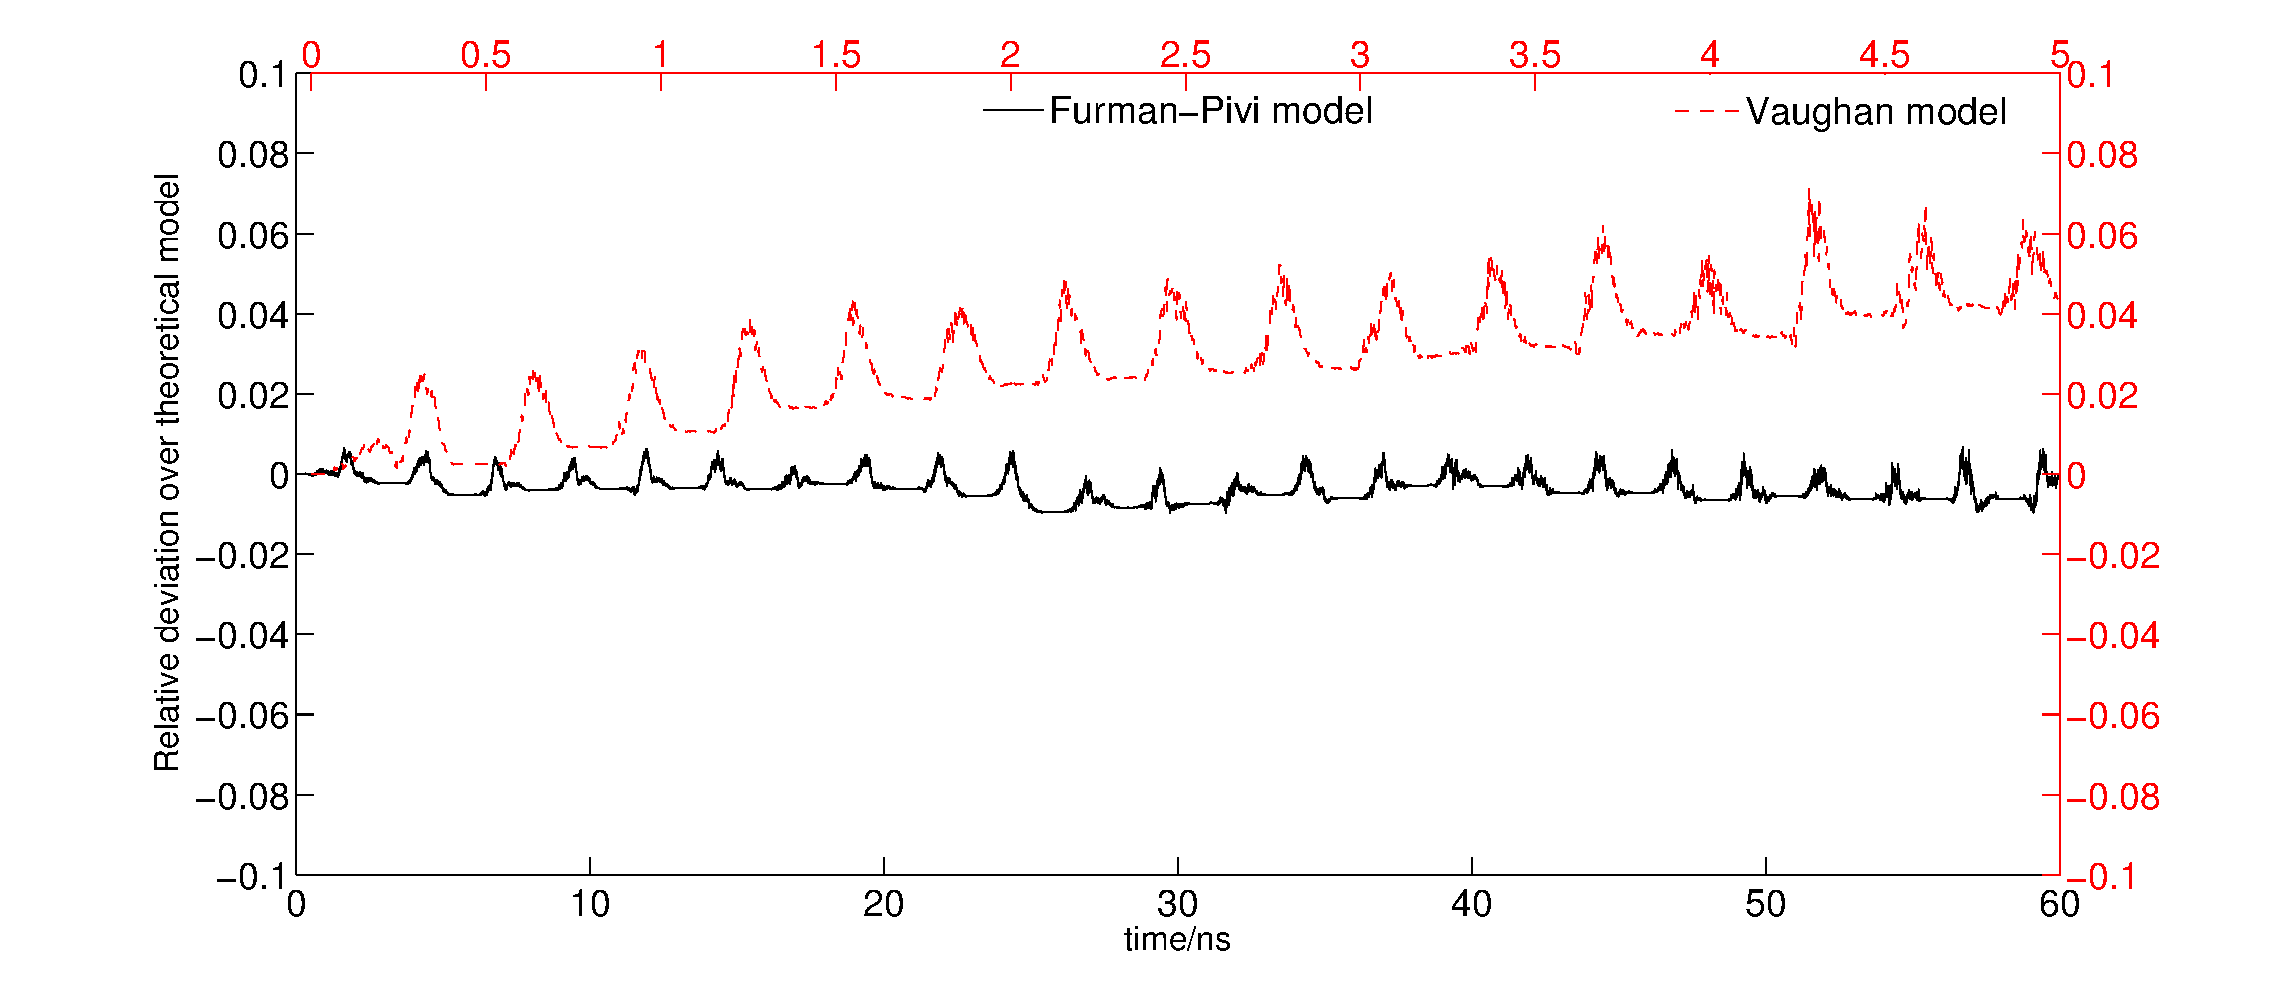
\includegraphics[width=0.9\textwidth]{models_comp_const_part.pdf}
\end{center}
\end{figure}
\item Relative deviations of simulation results over theoretical predicted values (re-normalize to const. simulation particle)
\end{itemize}
\end{frame} % to enforce entries in the table of contents
\section{Preliminary results}
\subsection{Dark Current Simulation on CTF3 Gun}
\begin{frame}
\frametitle{ANIMATION OF DARK CURRENT SIMULATION}
\begin{itemize}
\item We add a post processing feature which shows the origin positions and phase of dark current particles which are alive beyond user specified positions
\item \href{run:alivetest.avi}{\underline{Animation of CTF3 gun} }%\includegraphics{film still}}
\end{itemize}
\end{frame}
\subsection{Multipacting simulation on Cyclotron Cavity}
\begin{frame}[allowframebreaks]
\frametitle{Multipacting of CYCIAE-100MeV Cyclotron}
\begin{itemize}
\item We perform a parameter scan on the phase lag of RF cavity to select prone multipacting phase
\item Preliminary results only on full RF power case, further extension needed to evaluate prone multipacting conditions on different power level  
\end{itemize}
\begin{columns}
\begin{column}[t]{6.cm}
\begin{figure}[H]
\begin{center}
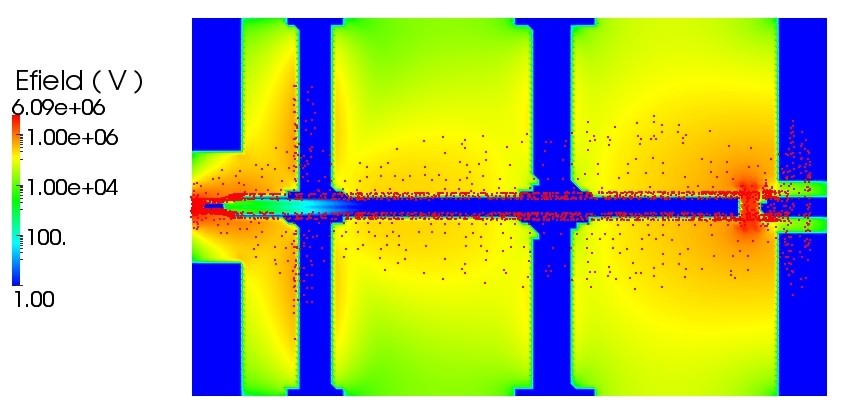
\includegraphics[width=1.\textwidth]{initial_field_particle.jpg}
\end{center}
\end{figure}
\end{column}
\begin{column}[t]{6.cm}
\begin{figure}[H]
\begin{center}
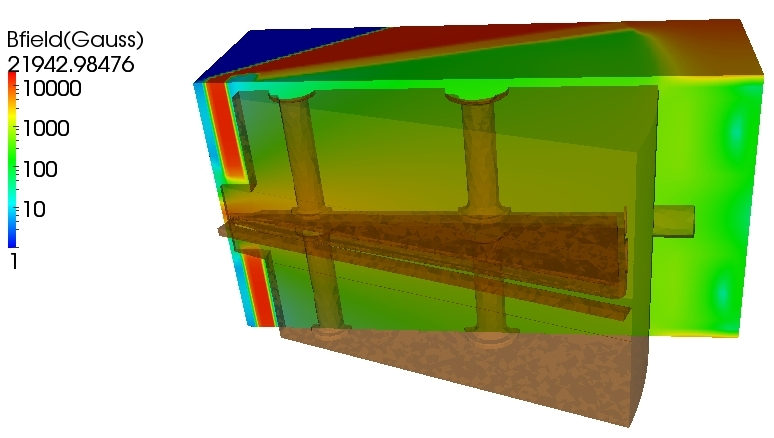
\includegraphics[width=1.\textwidth]{Bfield_Cavity.jpg}
\end{center}
\end{figure}
\end{column}
\end{columns}
\begin{itemize}
\item The secondary emission curve for copper varies for different surface treatments \cite{experiment}:
\begin{figure}[H]
\begin{center}
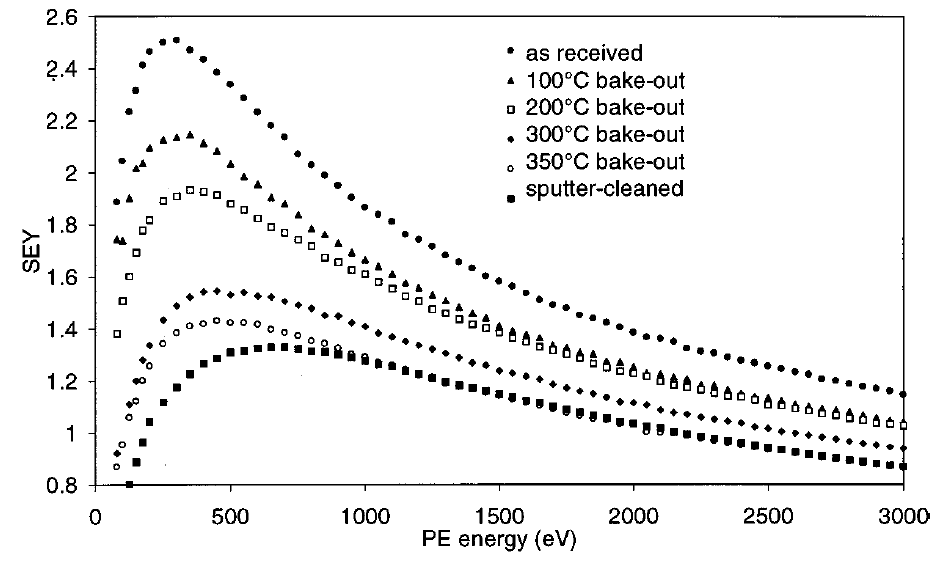
\includegraphics[width=0.7\textwidth]{SEY.png}
\end{center}
\end{figure}
\end{itemize}
\begin{itemize}
\item The secondary emission curve we use in parameter scan is:
\begin{figure}[H]
\begin{center}
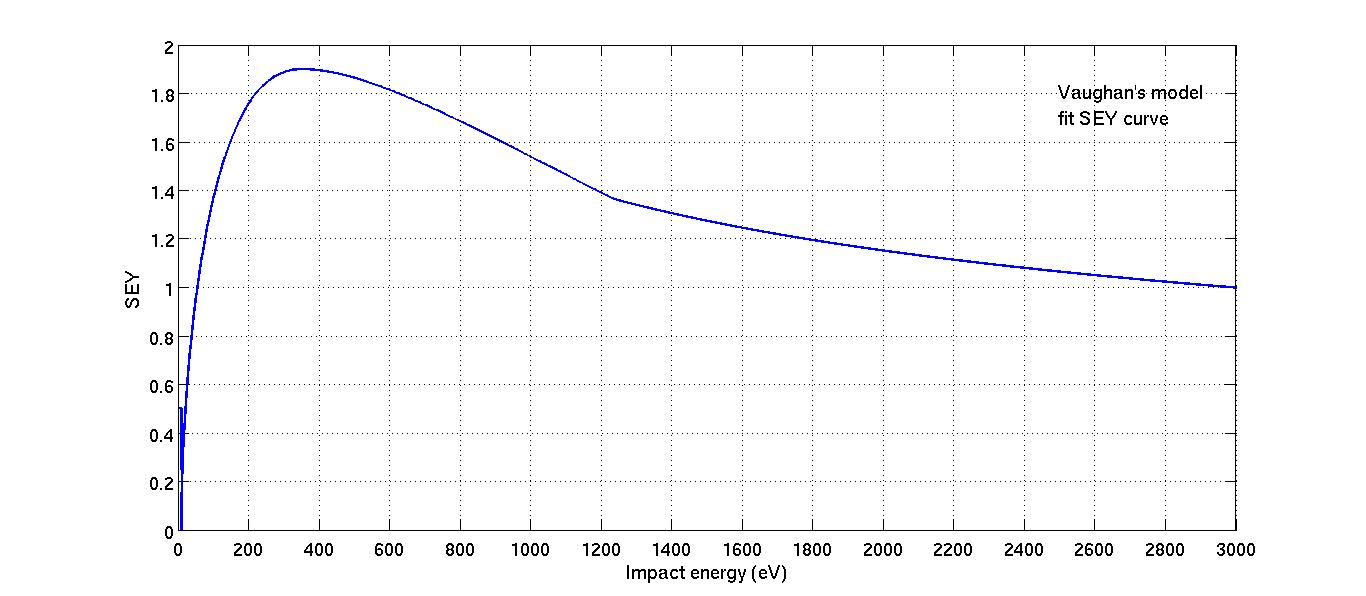
\includegraphics[width=1\textwidth]{SEY_used.jpg}
\end{center}
\end{figure}
\item Multiplication within 1 RF cycle has been observed:
\begin{figure}[H]
\begin{center}
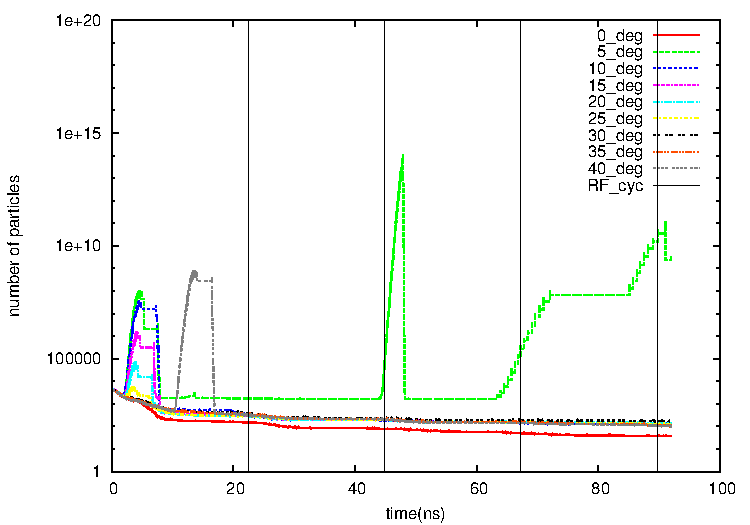
\includegraphics[width=0.7\textwidth]{para_scan1.pdf}
\end{center}
\end{figure}
\item Periodical multipacting with multiplication period $1\times \text{RF cycle}$ and  $3\times \text{RF cycle}$ has also been observed:
\begin{figure}[H]
\begin{center}
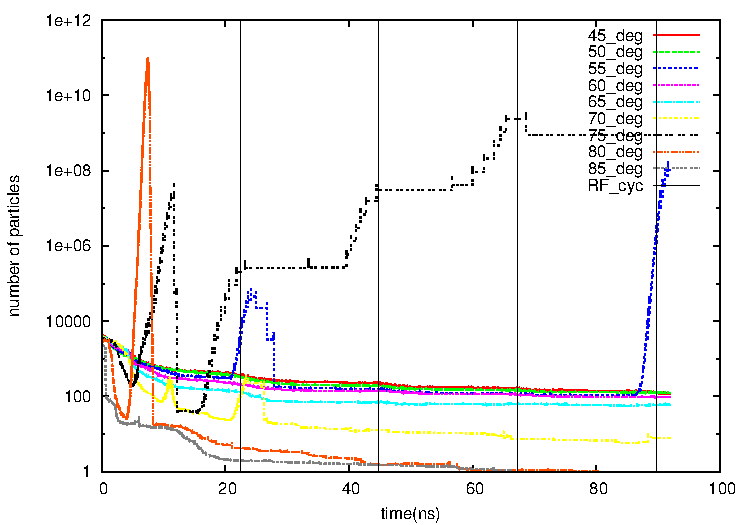
\includegraphics[width=0.7\textwidth]{para_scan2.pdf}
\end{center}
\end{figure}
\item Hot spot: \href{run:cyctest.avi}{\underline{Animation of hot spot where particle hit the surface} }%\includegraphics{film still}}
\item Dumped for each 100 time steps (0.4ns)
\begin{figure}[H]
\begin{center}
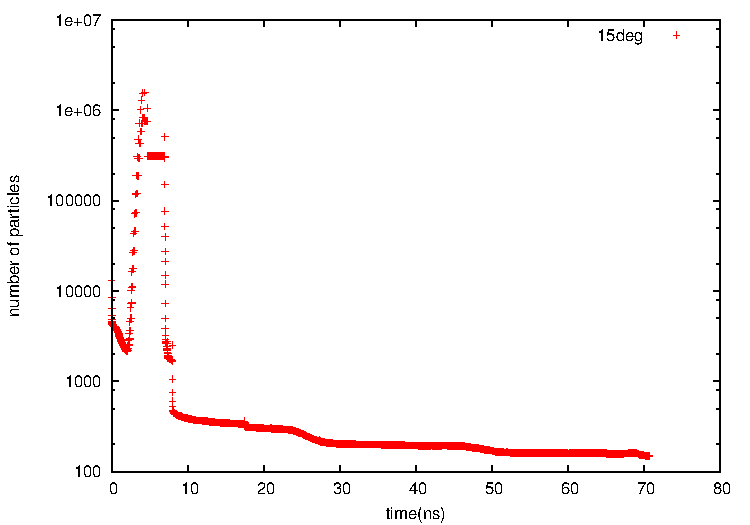
\includegraphics[width=0.7\textwidth]{const_test.pdf}
\end{center}
\end{figure}
\end{itemize}
\end{frame}
\section*{Conclusions}
\begin{frame}
\begin{itemize}
\item We have modeled, implemented the dark current module and also benchmarked the multipacting module of OPAL  
\item Preliminary study cases have shown the capability of OPAL on the dark current and multipacting study
\end{itemize}
\end{frame}
\begin{frame}
\frametitle{Future Plan}
\begin{itemize}
\item Parallelization scheme choices and H5FED/H5HUT geometry format
\item Further multipacting study on different RF power level is useful to predict and understand the behavior of the cavities of CYCIAE-100
\item Obtain hot spots in different RF power level by simulations to determine the position where a special surface treatment is needed to suppress multipacting
\item Preparing the documents and papers
\end{itemize}
\end{frame}
\begin{frame}
\frametitle{ACKNOWLEDGEMENT}
Here we want to express our deep appreciation to Dr. Mike Seidel, Dr. Benedikt Oswald, Dr. Lukas Stingelin.
We'd like thank our colleagues Ch. Kraus, Hua Guo, A. Gsell, M. Wittberger in AMAS group, for the fruitful discussions and good ideas. 
\end{frame}
\begin{frame}[allowframebreaks]
\frametitle{REFERENCES}
\begin{thebibliography}{99}
\bibitem[V.E. Boria et al] {SPACE}V.E. Boria, B. Gimeno, C. Vicente, A.M. P�rez,
G. Torregrosa, A. Coves, A. �lvarez, F. Quesada, IMS 2007 Workshop WMH 
High Power Issues of Microwave Filter Design and Realization.

\bibitem[A.Moretti et al]{Linac} A.Moretti et al., Proc. of LINAC 2004, L�beck, Germany
\bibitem[J. Cherix, P. Sigg]{cyclotron} J. Cherix, P. Sigg, PSI - Scientific and Technical Report 2004 / Volume VI
\bibitem[F.L.Krawczyk] {coderv} F.L.Krawczyk, The 10 th Workshop on RF Superconductivity, 2001, Tsukuba, Japan
\bibitem[D.Sunday's]{LT} D. Sunday,
 available online on:\\ \href{http://softsurfer.com/Archive/algorithm\_0105/algorithm\_0105.htm}{http://softsurfer.com/Archive/algorithm\_0105/algorithm\_0105.htm}
\bibitem[R. H. Fowler, L. Nordheim]{FN} R. H. Fowler and L. Nordheim, 
Proc. R. Soc. London, Ser. A 119, 173 (1928)
\bibitem[J. H. Han]{DE} J. H. Han, PhD Thesis, Desy, 2005 available online on \href{http://www-library.desy.de/preparch/desy/thesis/desy-thesis-05-045.pdf}{http://www-library.desy.de/preparch/desy/thesis/desy-thesis-05-045.pdf}
\bibitem[Y. Feng and J. P. Verboncoeur's paper]{BC} Y. Feng and J. P. Verboncoeur,
Phys.Plasmas 13, 073105 (2006)
\bibitem[A. Adelmann, P. Arbenz and Y. Ineichen]{SV} A. Adelmann, P. Arbenz and Y. Ineichen, 
J. Comp. Phys, 229 (12): 4554-4566 (2010)
\bibitem[M. A. Furman and M. Pivi]{SE} M. A. Furman and M. Pivi, 
 Phys. Rev. ST Accel. Beams 5, 124404 (2002)
\bibitem[S. Anza et al]{NS} S. Anza, C. Vicente, J. Gil, V. E. Boria, B. Gimeno, and D. Raboso, Phys. Plasmas 17, 062110 2010
\bibitem[I. Bojkoa et al]{experiment} I. Bojkoa, N. Hilleret and Ch. Scheuerlein, J. Vac. Sci. Technol. A, Vol. 18, No. 3, 2000


\end{thebibliography}
\end{frame}
\begin{frame}[allowframebreaks]
\frametitle{Appendix: Formulas for Non-Stationary Theory}
\begin{itemize}
\item The solution of \eqref{nposition} when electron hit the plates, i.e., when $\xi(\varphi,\varphi_0,u)=\lambda \ \text{or} \ 0$, is a probabilistic number, as the emission velocity $u$ is a random number 
\item The probability density of the least root(on variable $\tau$) of equation \eqref{nposition} can be expressed by the known distribution $f_u=\frac{uv^2_{\omega}}{v^2_t}\exp{\left(-\frac{u^2v^2_{\omega}}{2v^2_t}\right)}$ of velocity $u$:
 \begin{equation*}
G(\tau|\varphi_0;\lambda)=\left| \frac{\mathrm{d}g(\tau|\varphi_0;\lambda)}{\mathrm{d}\tau} \right| f_u[g(\tau|\varphi_0;\lambda)] \label{gdsdef}
\end{equation*}
\begin{equation*}
G(\tau|\varphi_0;0)=\left| \frac{\mathrm{d}g(\tau|\varphi_0;0)}{\mathrm{d}\tau} \right| f_u[g(\tau|\varphi_0;0)] \label{gssdef}
\end{equation*}
where, $u=g(\tau|\varphi_0;\lambda)$ and $u=g(\tau|\varphi_0;0)$ respectively (monotonic function)
\end{itemize}
\begin{itemize}
\item Emission rate (electrons/radian) in plate $U/D$ at phase $\varphi$:
\begin{flalign*}
C_U(\varphi)&=\int_0^\varphi C_D(\varphi')G_{ds,D}(\varphi-\varphi'|\varphi')\delta_{ds,D}(\varphi-\varphi'|\varphi')\mathrm{d}\varphi'\nonumber \\
&+\int_0^\varphi C_U(\varphi')G_{ss,U}(\varphi-\varphi'|\varphi')\delta_{ss,U}(\varphi-\varphi'|\varphi')\mathrm{d}\varphi'+\Psi_U(\varphi)
\end{flalign*}
\begin{flalign*}
C_D(\varphi)&=\int_0^\varphi C_D(\varphi')G_{ss,D}(\varphi-\varphi'|\varphi')\delta_{ss,D}(\varphi-\varphi'|\varphi')\mathrm{d}\varphi'\nonumber \\
&+\int_0^\varphi C_U(\varphi')G_{ds,U}(\varphi-\varphi'|\varphi')\delta_{ds,U}(\varphi-\varphi'|\varphi')\mathrm{d}\varphi'+\Psi_D(\varphi)
\end{flalign*}
\item Volterra integral equations of the second
\end{itemize}
\begin{itemize}
\item Impact rate (electrons/radian) in plate $U/D$ at phase $\varphi$:
\begin{flalign*}
I_U(\varphi)=&\int_0^\varphi C_D(\varphi')G_{ds,D}(\varphi-\varphi'|\varphi')\mathrm{d}\varphi'\nonumber \\
&+\int_0^\varphi C_U(\varphi')G_{ss,U}(\varphi-\varphi'|\varphi')\mathrm{d}\varphi'
\end{flalign*}
\begin{flalign*}
I_D(\varphi)=&\int_0^\varphi C_D(\varphi')G_{ss,D}(\varphi-\varphi'|\varphi')\mathrm{d}\varphi'\nonumber \\
&+\int_0^\varphi C_U(\varphi')G_{ds,U}(\varphi-\varphi'|\varphi')\mathrm{d}\varphi'
\end{flalign*}
\item Number of particles:
\begin{flalign*}
N(\varphi)=&\int_0^\varphi \left(C_U(\varphi')+C_D(\varphi')-I_U(\varphi')-I_D(\varphi')\right)\mathrm{d}\varphi'
\end{flalign*}
\end{itemize}
\end{frame}
\end{document}
